\chapter{Artefakte der Analyse-Phase}

\begin{figure}[ht]
\centering
%trim=l b r t  	This option will crop the imported image by l from the left, b from the bottom, r from the right, and t  from the top. Where l, b, r and t are lengths. 
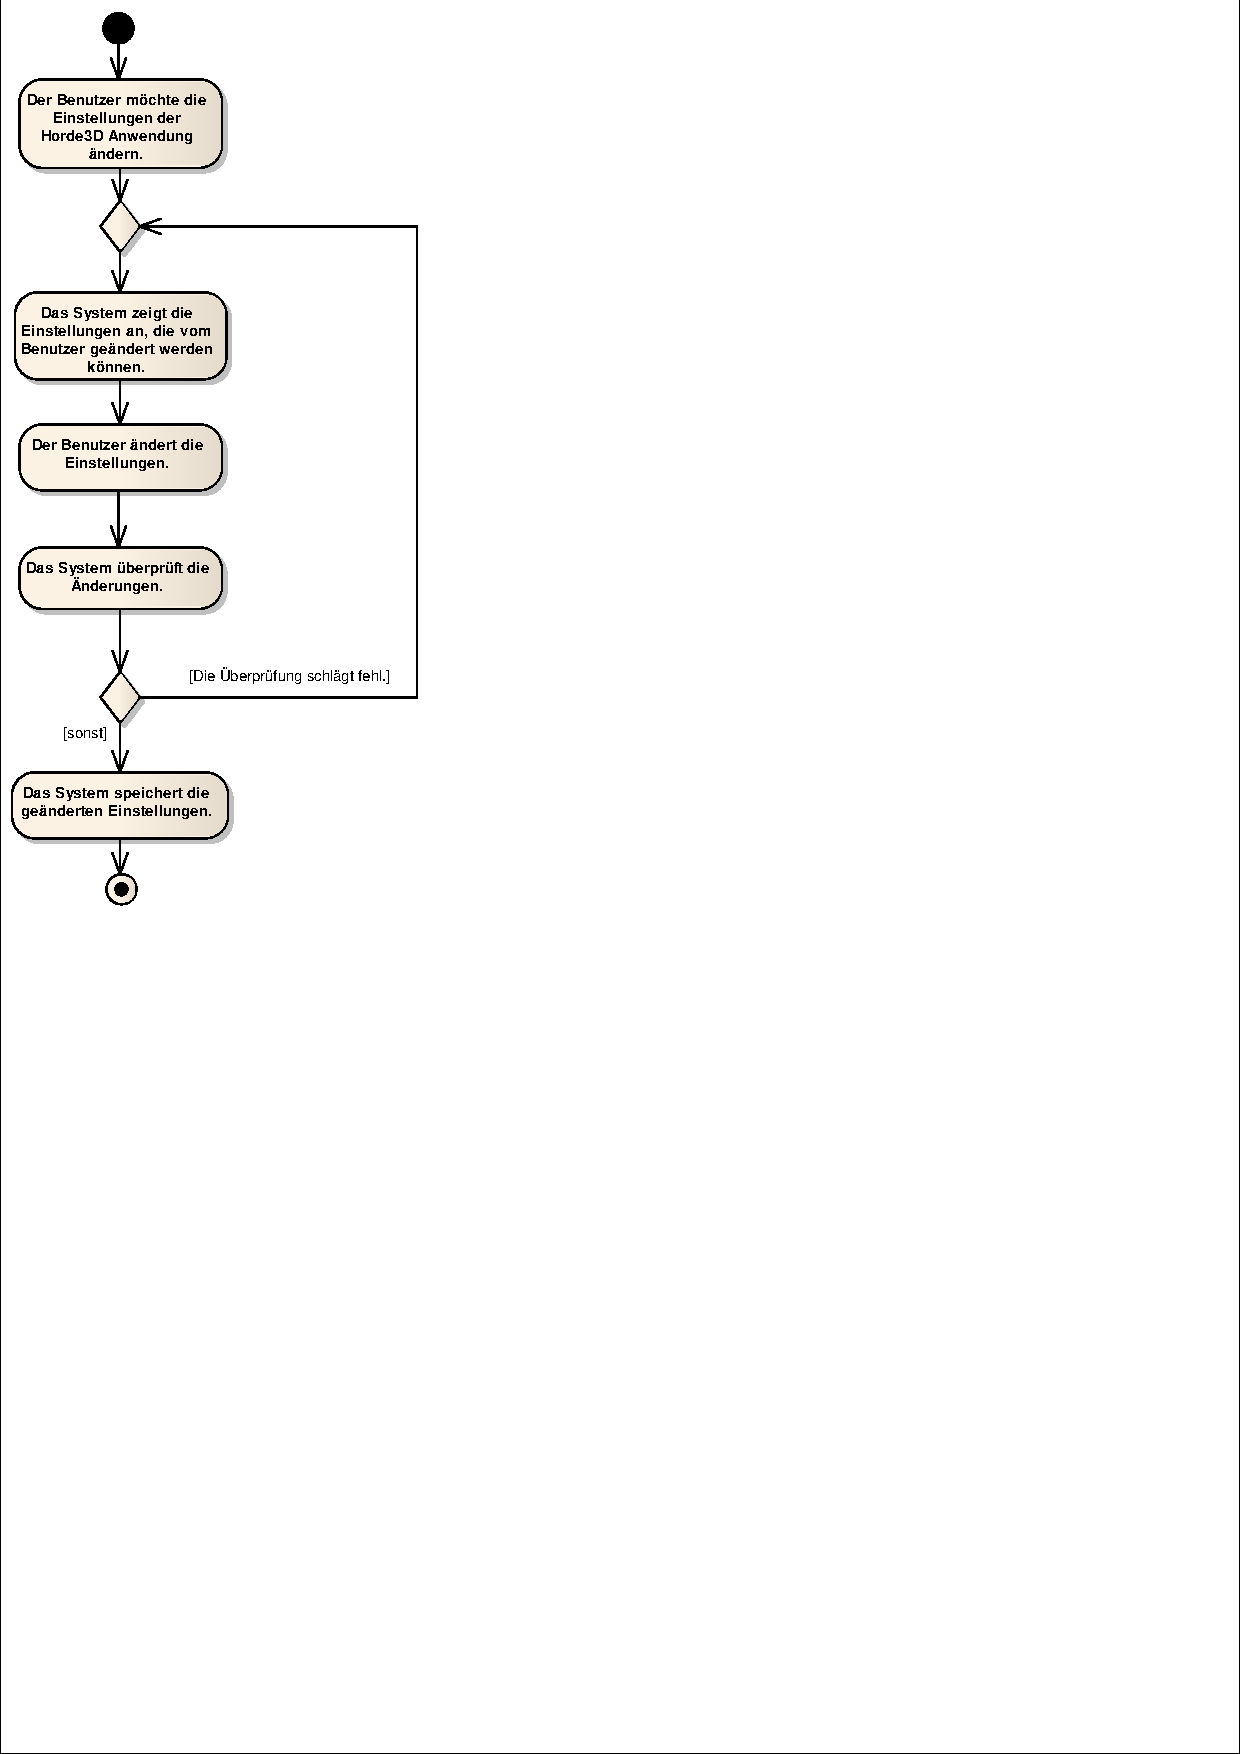
\includegraphics[trim = 1mm 140mm 135mm 1mm, clip, scale=0.7]{images/UseCase_EinstellungenAendern.pdf}
\caption{Aktivit�tsdiagramm f�r den Anwendungsfall "`Einstellungen �ndern"'}\label{fig:ucEinstellungenAendern}
\end{figure}

\begin{figure}[htp]
\centering
%trim=l b r t  	This option will crop the imported image by l from the left, b from the bottom, r from the right, and t  from the top. Where l, b, r and t are lengths. 
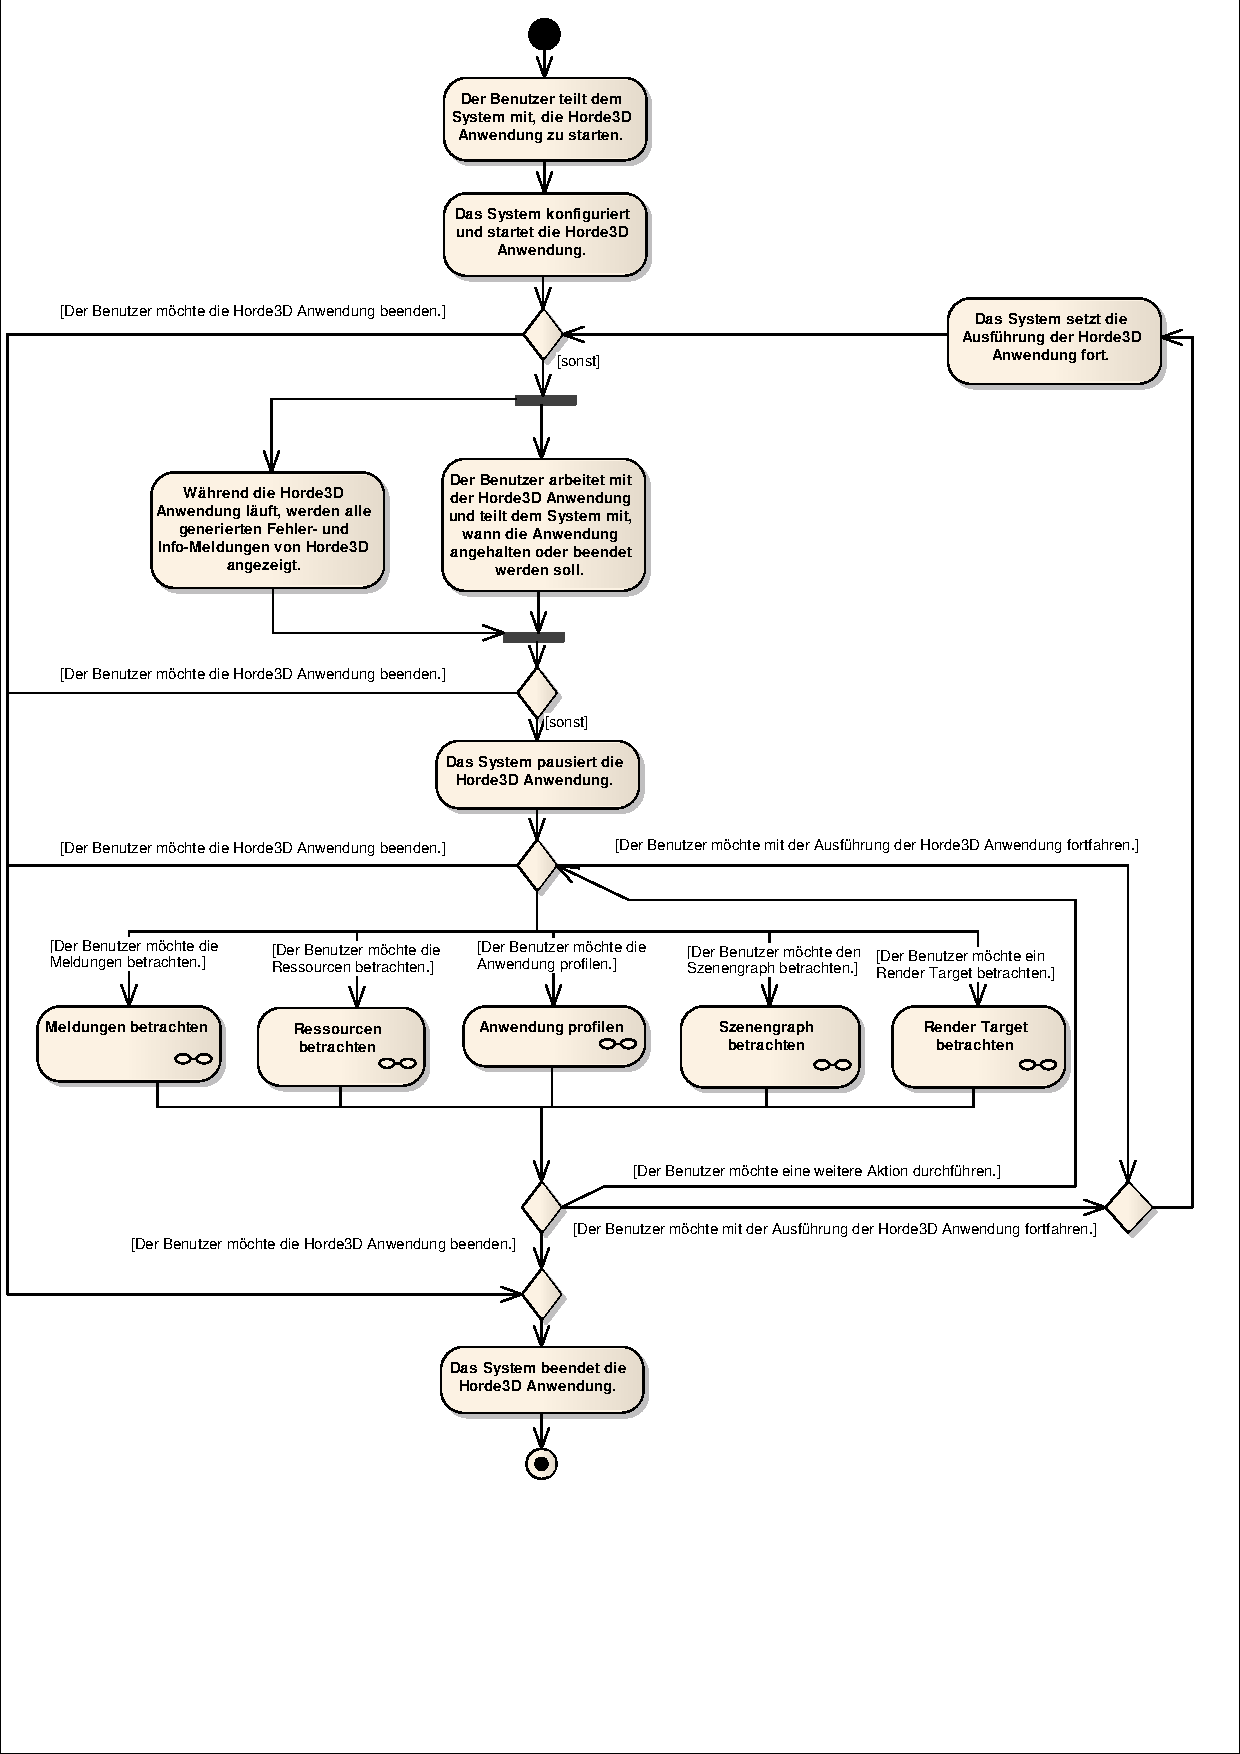
\includegraphics[trim = 1mm 45mm 5mm 1mm, clip, scale=0.7]{images/UseCase_AnwendungAusfuehren.pdf}
\caption{Aktivit�tsdiagramm f�r den Anwendungsfall "`Anwendung ausf�hren"'}\label{fig:ucAnwendungAusfuehren}
\end{figure}

\begin{figure}[ht]
\centering
%trim=l b r t  	This option will crop the imported image by l from the left, b from the bottom, r from the right, and t  from the top. Where l, b, r and t are lengths. 
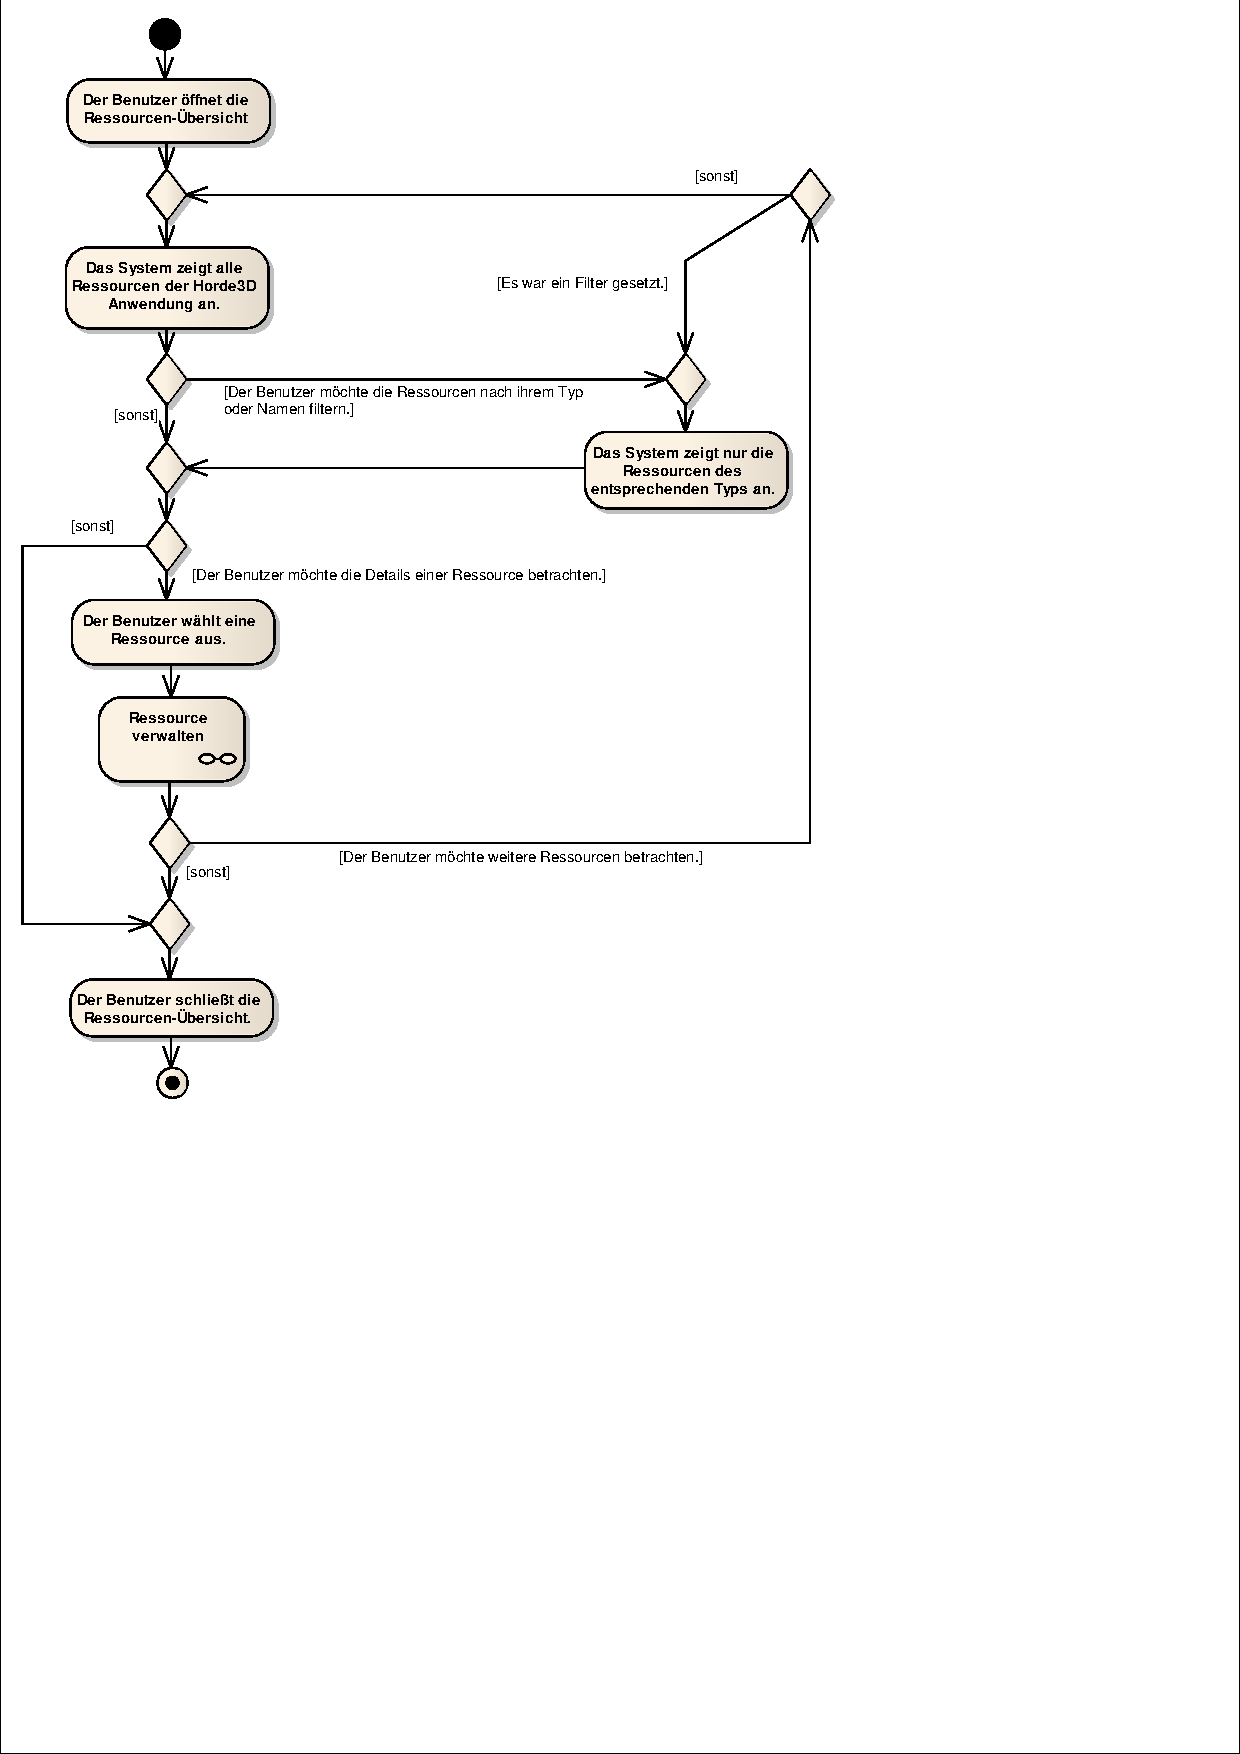
\includegraphics[trim = 1mm 110mm 60mm 1mm, clip, scale=0.7]{images/UseCase_RessourcenBetrachten.pdf}
\caption{Aktivit�tsdiagramm f�r den Anwendungsfall "`Ressourcen betrachten"'}\label{fig:ucRessourcenBetrachten}
\end{figure}

\begin{figure}[ht]
\centering
%trim=l b r t  	This option will crop the imported image by l from the left, b from the bottom, r from the right, and t  from the top. Where l, b, r and t are lengths. 
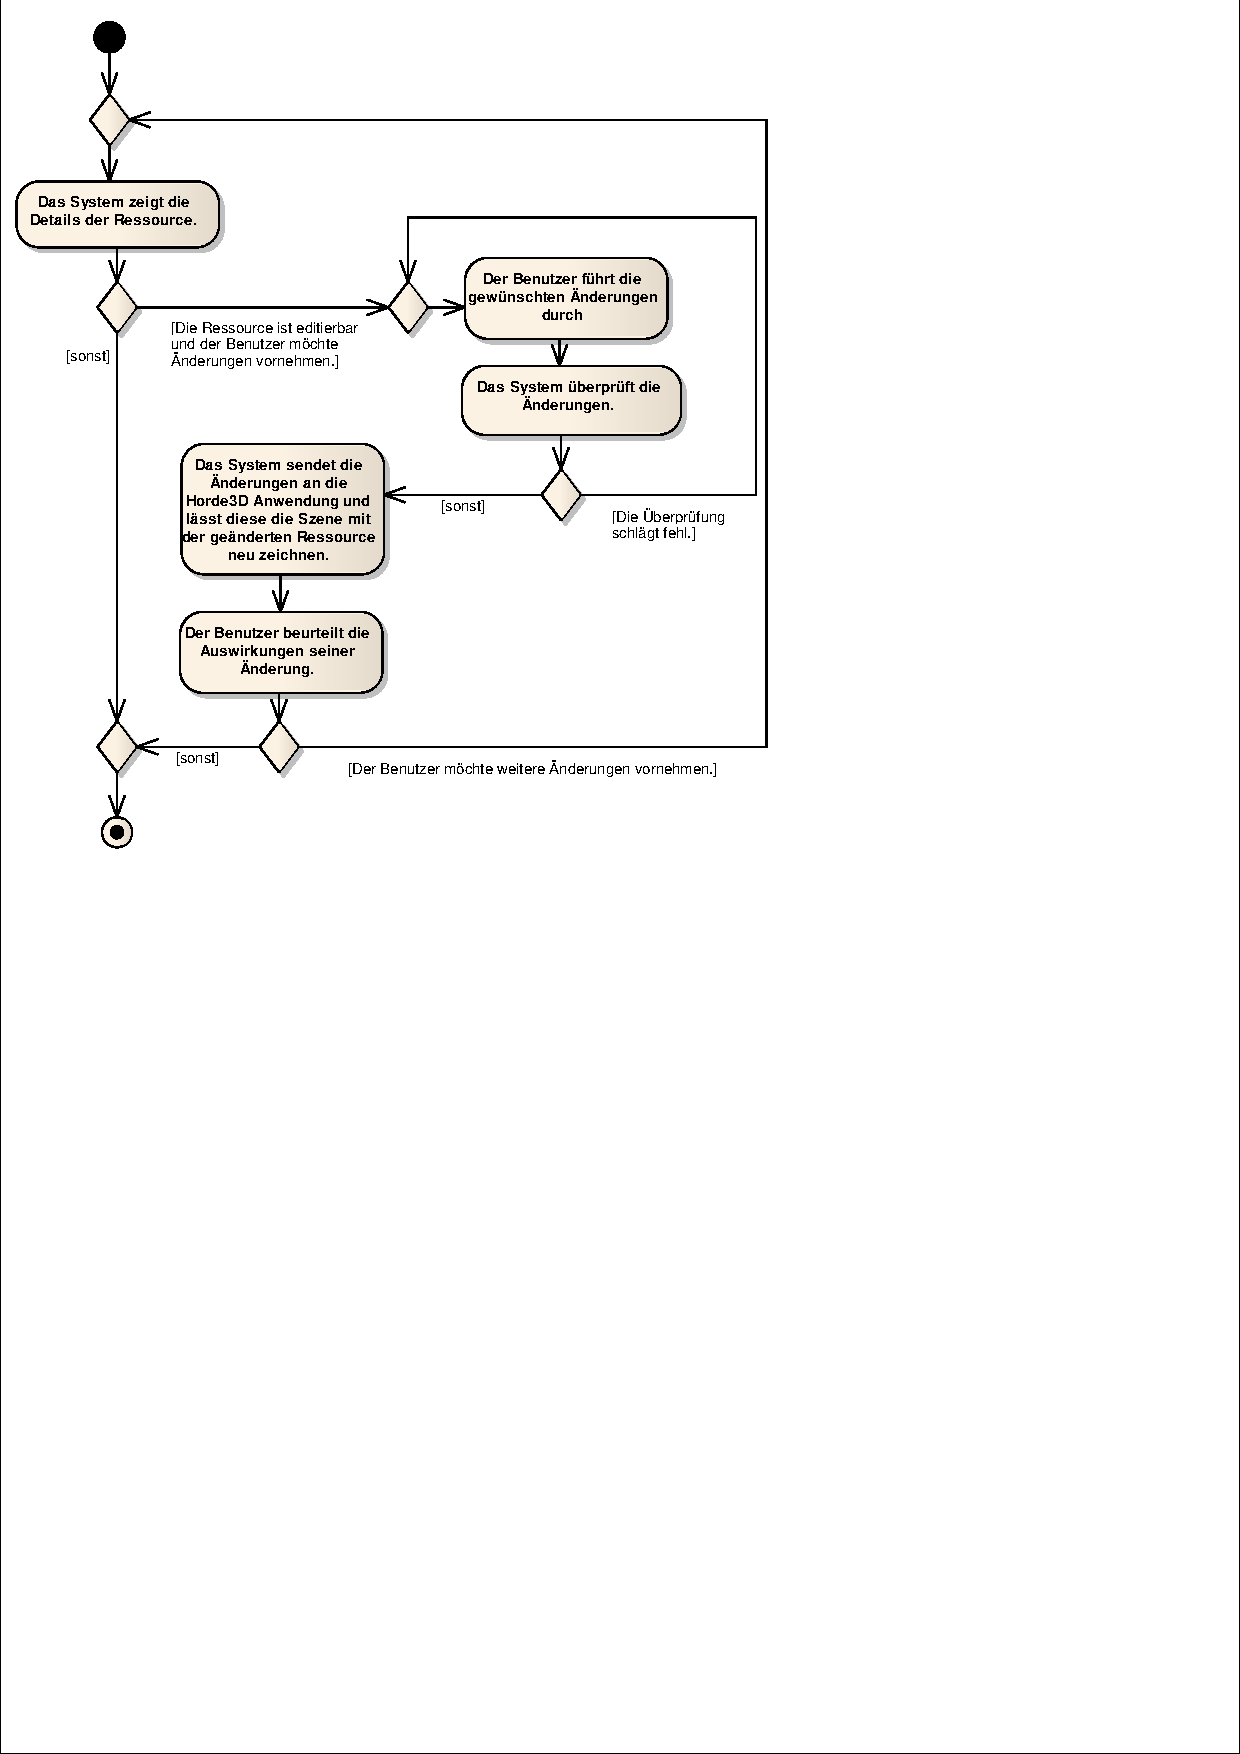
\includegraphics[trim = 1mm 150mm 80mm 1mm, clip, scale=0.7]{images/UseCase_RessourceVerwalten.pdf}
\caption{Aktivit�tsdiagramm f�r den Anwendungsfall "`Ressource verwalten"'}\label{fig:ucRessourceVerwalten}
\end{figure}

\begin{figure}[htp]
\centering
%trim=l b r t  	This option will crop the imported image by l from the left, b from the bottom, r from the right, and t  from the top. Where l, b, r and t are lengths. 
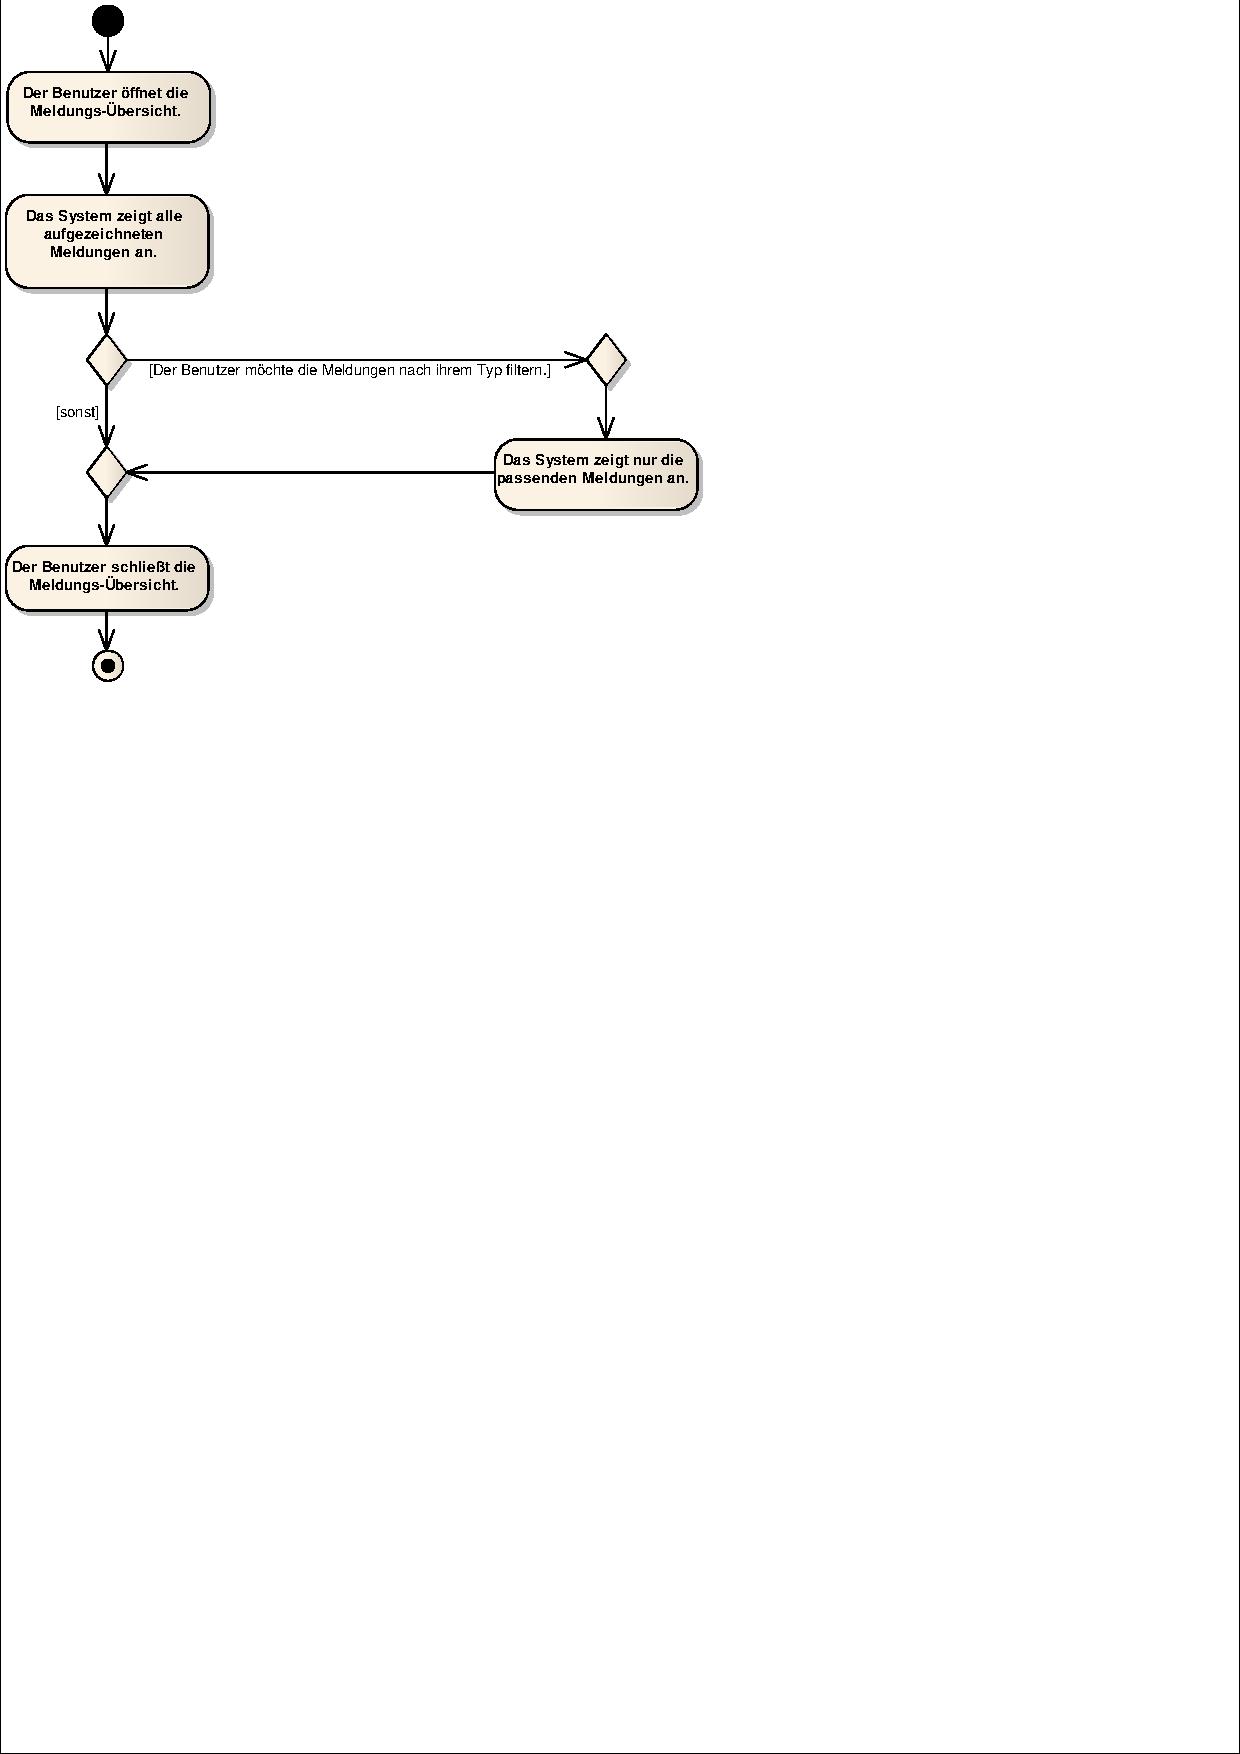
\includegraphics[trim = 1mm 180mm 90mm 1mm, clip, scale=0.7]{images/UseCase_MeldungenBetrachten.pdf}
\caption{Aktivit�tsdiagramm f�r den Anwendungsfall "`Meldungen betrachten"'}\label{fig:ucMeldungenBetrachten}
\end{figure}

\begin{figure}[htp]
\centering
%trim=l b r t  	This option will crop the imported image by l from the left, b from the bottom, r from the right, and t  from the top. Where l, b, r and t are lengths. 
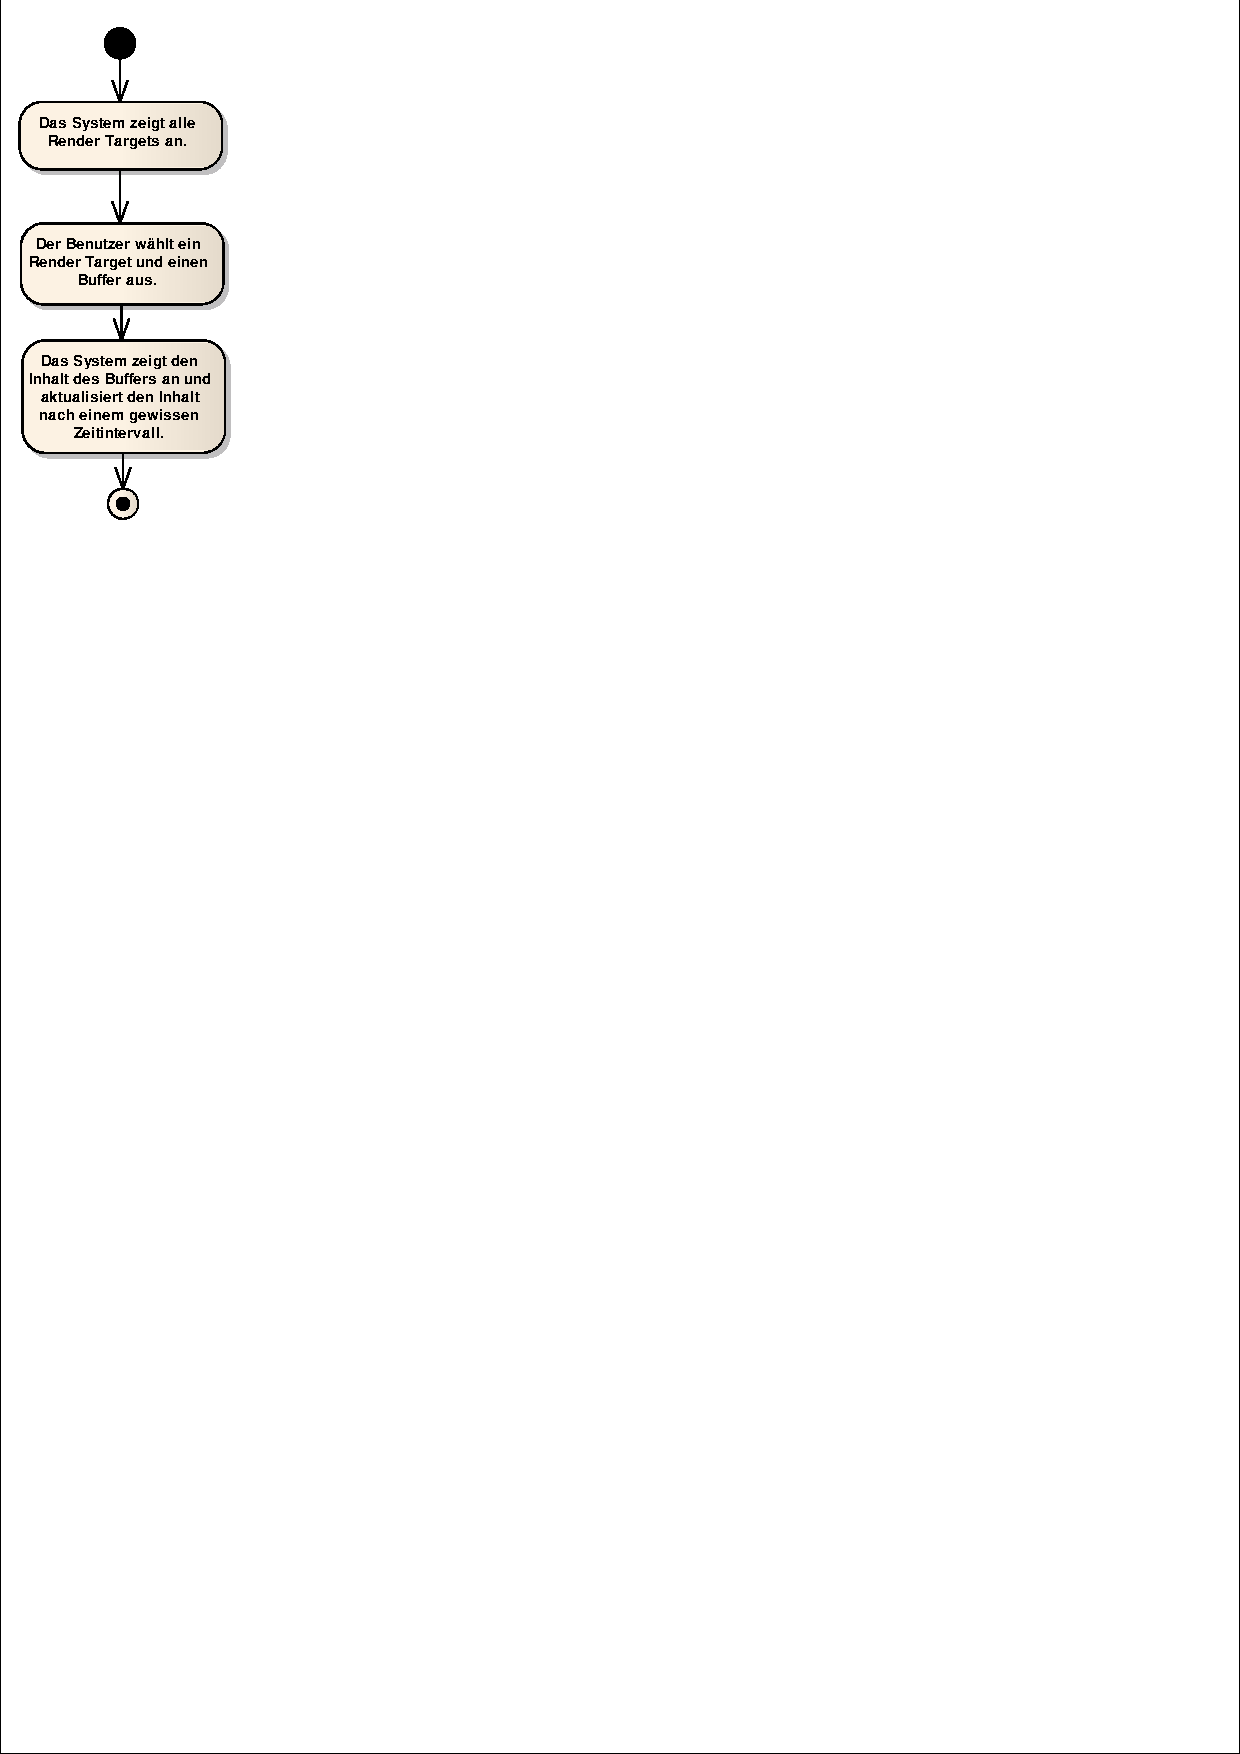
\includegraphics[trim = 1mm 205mm 150mm 1mm, clip, scale=0.7]{images/UseCase_RenderTargetBetrachten.pdf}
\caption{Aktivit�tsdiagramm f�r den Anwendungsfall "`Render Target betrachten"'}\label{fig:ucRenderTargetBetrachten}
\end{figure}

\begin{figure}[htp]
\centering
%trim=l b r t  	This option will crop the imported image by l from the left, b from the bottom, r from the right, and t  from the top. Where l, b, r and t are lengths. 
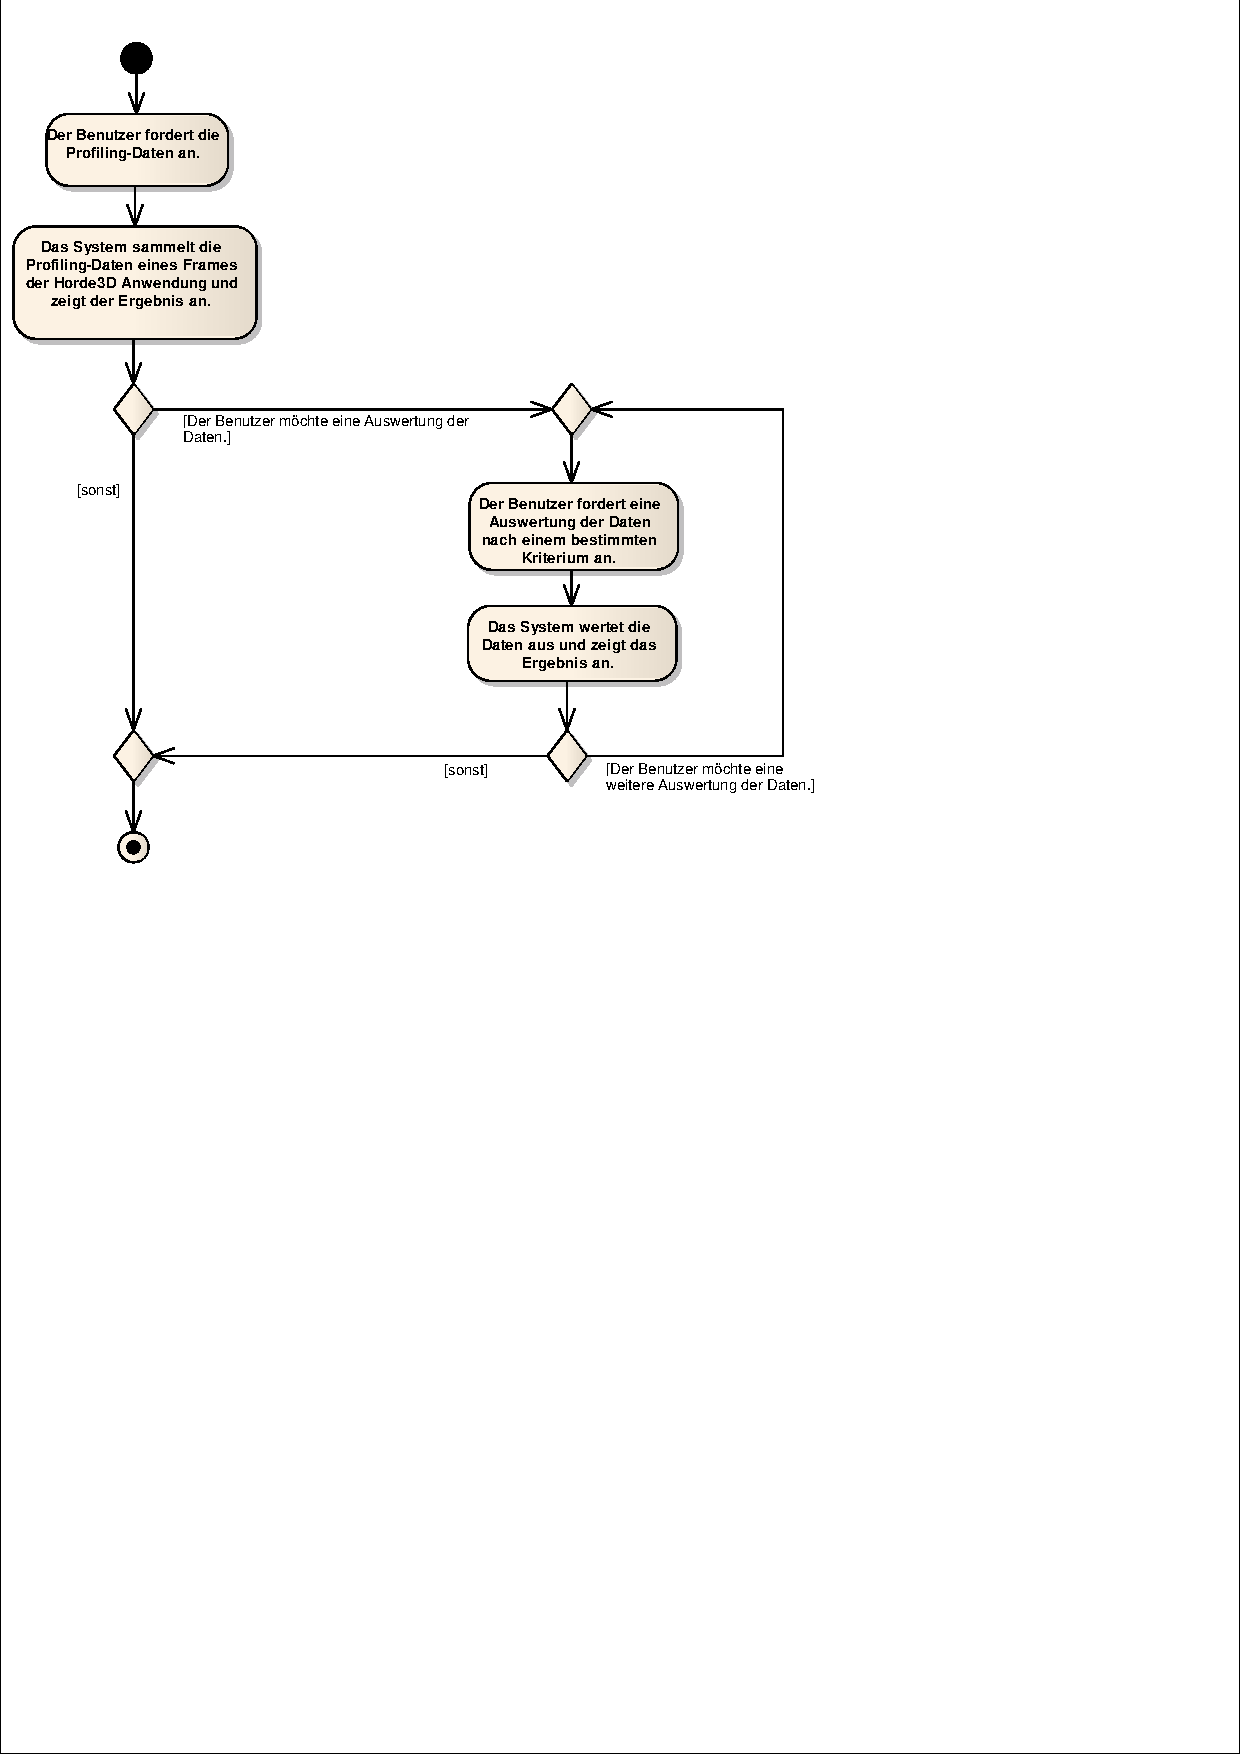
\includegraphics[trim = 1mm 150mm 60mm 1mm, clip, scale=0.7]{images/UseCase_AnwendungProfilen.pdf}
\caption{Aktivit�tsdiagramm f�r den Anwendungsfall "`Anwendung profilen"'}\label{fig:ucAnwendungProfilen}
\end{figure}

\begin{figure}[htp]
\centering
%trim=l b r t  	This option will crop the imported image by l from the left, b from the bottom, r from the right, and t  from the top. Where l, b, r and t are lengths. 
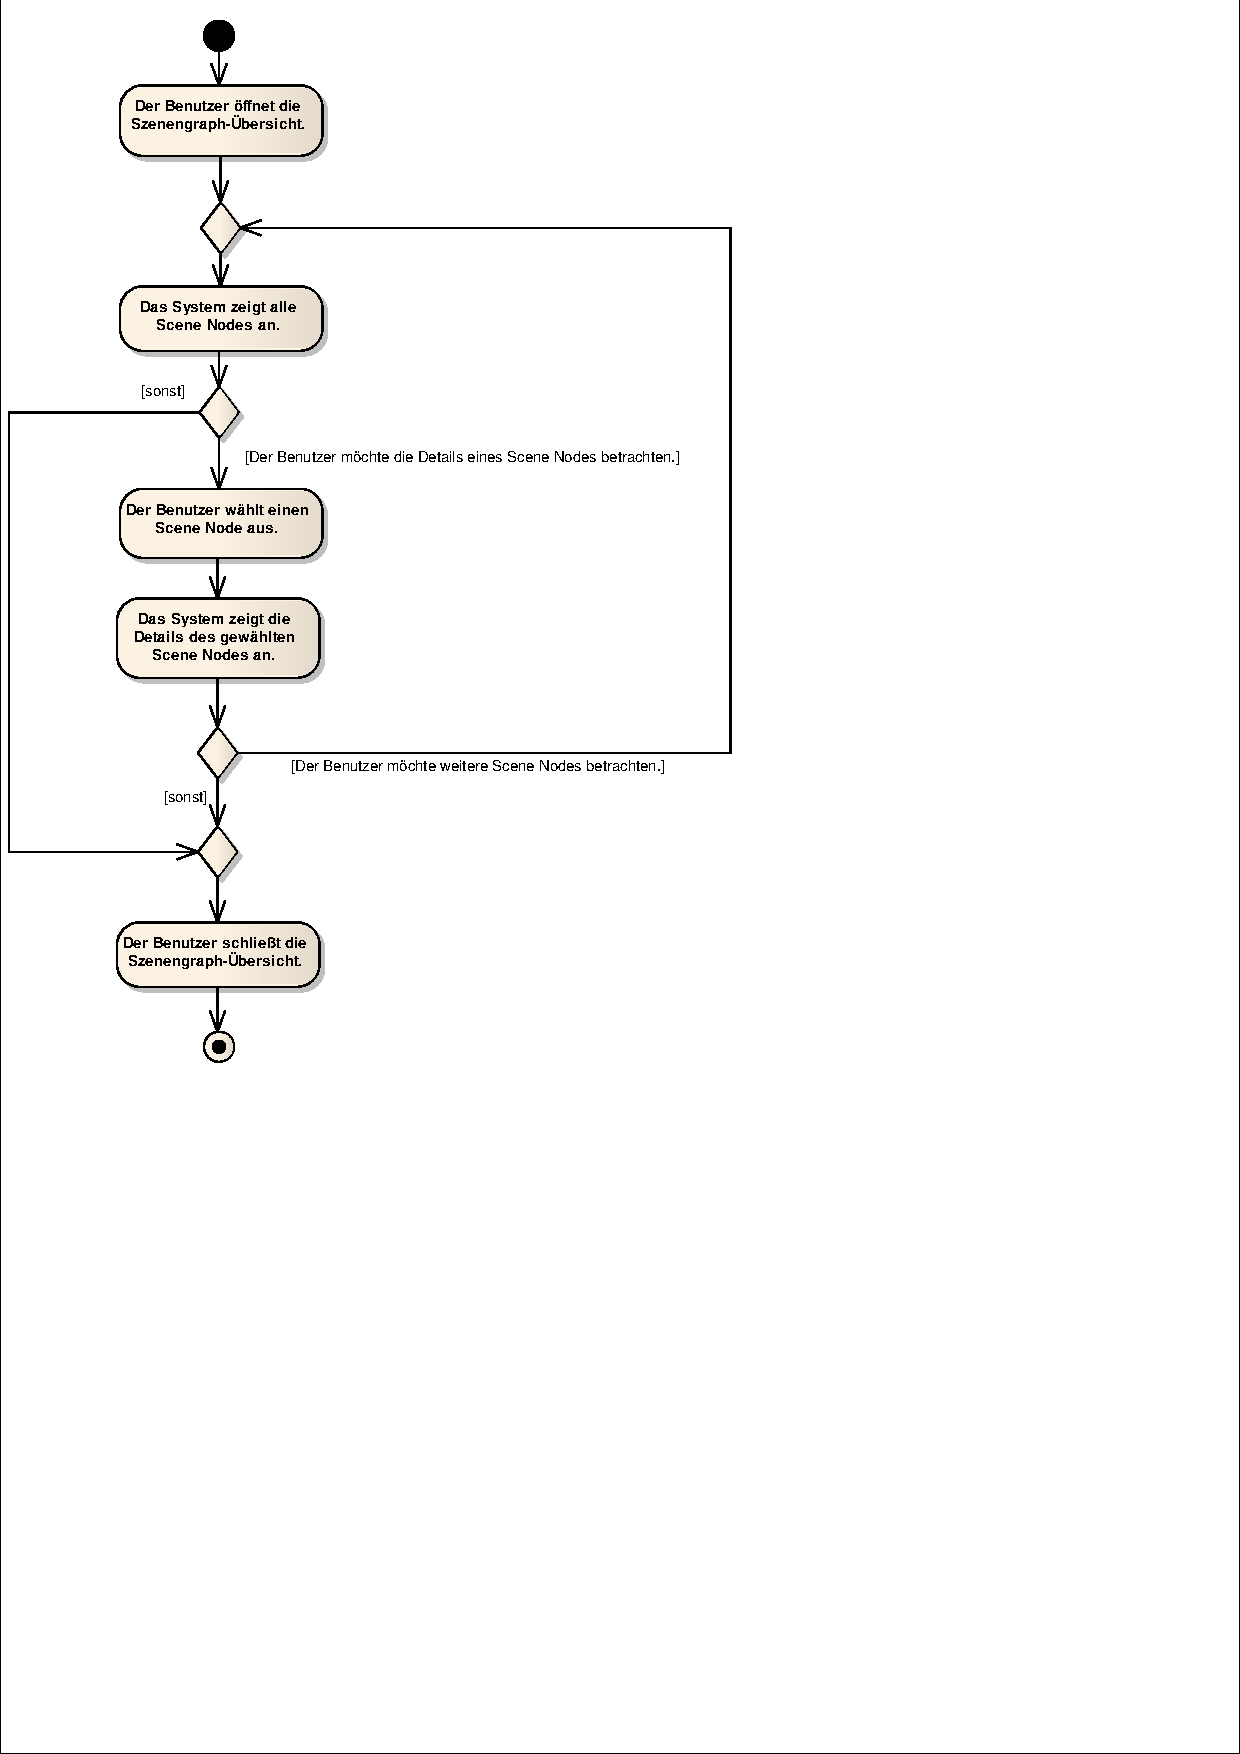
\includegraphics[trim = 1mm 115mm 70mm 1mm, clip, scale=0.7]{images/UseCase_SzenengraphBetrachten.pdf}
\caption{Aktivit�tsdiagramm f�r den Anwendungsfall "`Szenengraph betrachten"'}\label{fig:ucSzenengraphBetrachten}
\end{figure}

\begin{figure}[htp]
\centering
%trim=l b r t  	This option will crop the imported image by l from the left, b from the bottom, r from the right, and t  from the top. Where l, b, r and t are lengths. 
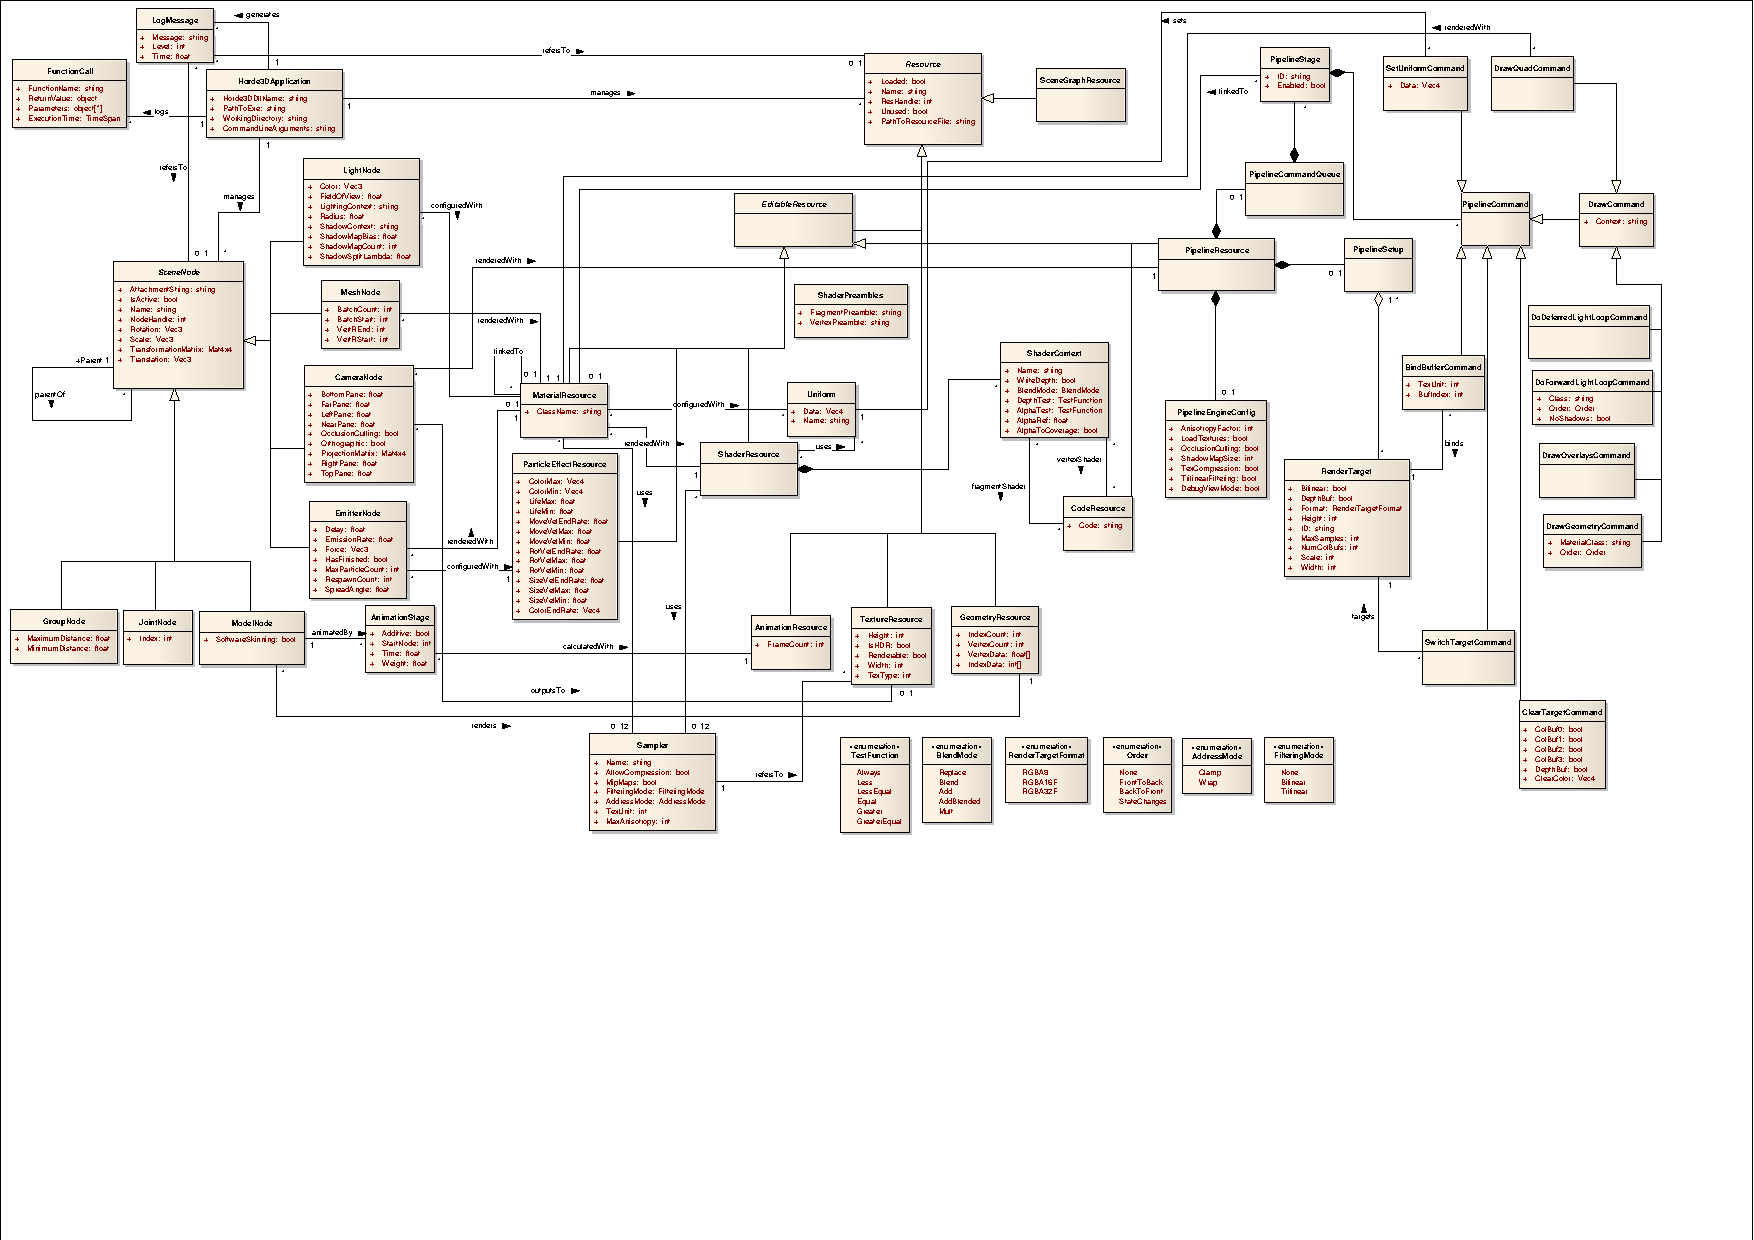
\includegraphics[trim = 1mm 65mm 15mm 1mm, clip, scale = 0.75, angle = 90]{images/DomainModel.pdf}
\caption{Das Konzeptmodell des \DevEnvs}\label{fig:domainModel}
\end{figure}

\chapter{Artefakte der Design-Phase}

\begin{figure}[htp]
\centering
%trim=l b r t  	This option will crop the imported image by l from the left, b from the bottom, r from the right, and t  from the top. Where l, b, r and t are lengths. 
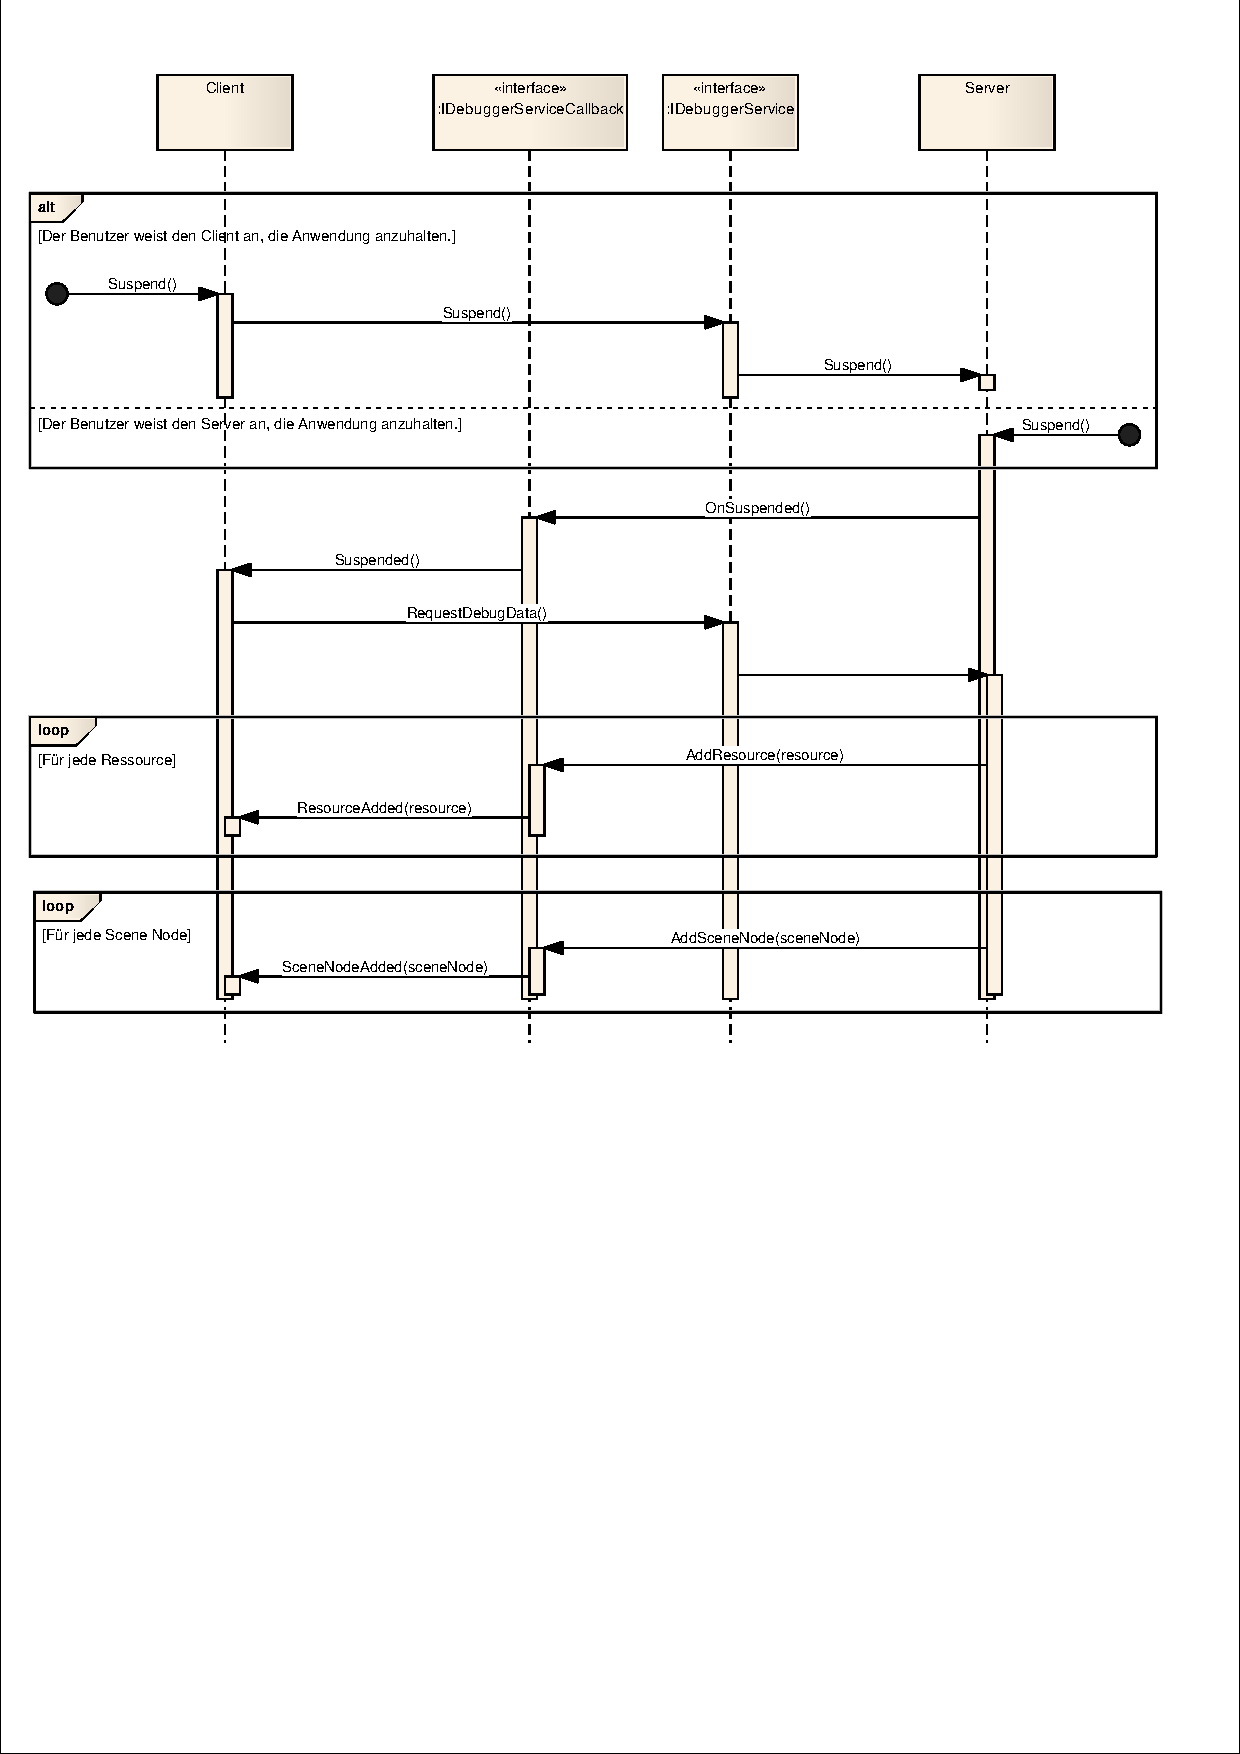
\includegraphics[trim = 5mm 120mm 5mm 10mm, clip,scale=0.7]{images/ClientServerCommunication.pdf}
\caption{Sequenzdiagramm f�r die Client-Server-Interaktionen beim Anhalten der Anwendung}\label{fig:ClientServerCommunication}
\end{figure}

\begin{figure}[htp]
\centering
%trim=l b r t  	This option will crop the imported image by l from the left, b from the bottom, r from the right, and t  from the top. Where l, b, r and t are lengths. 
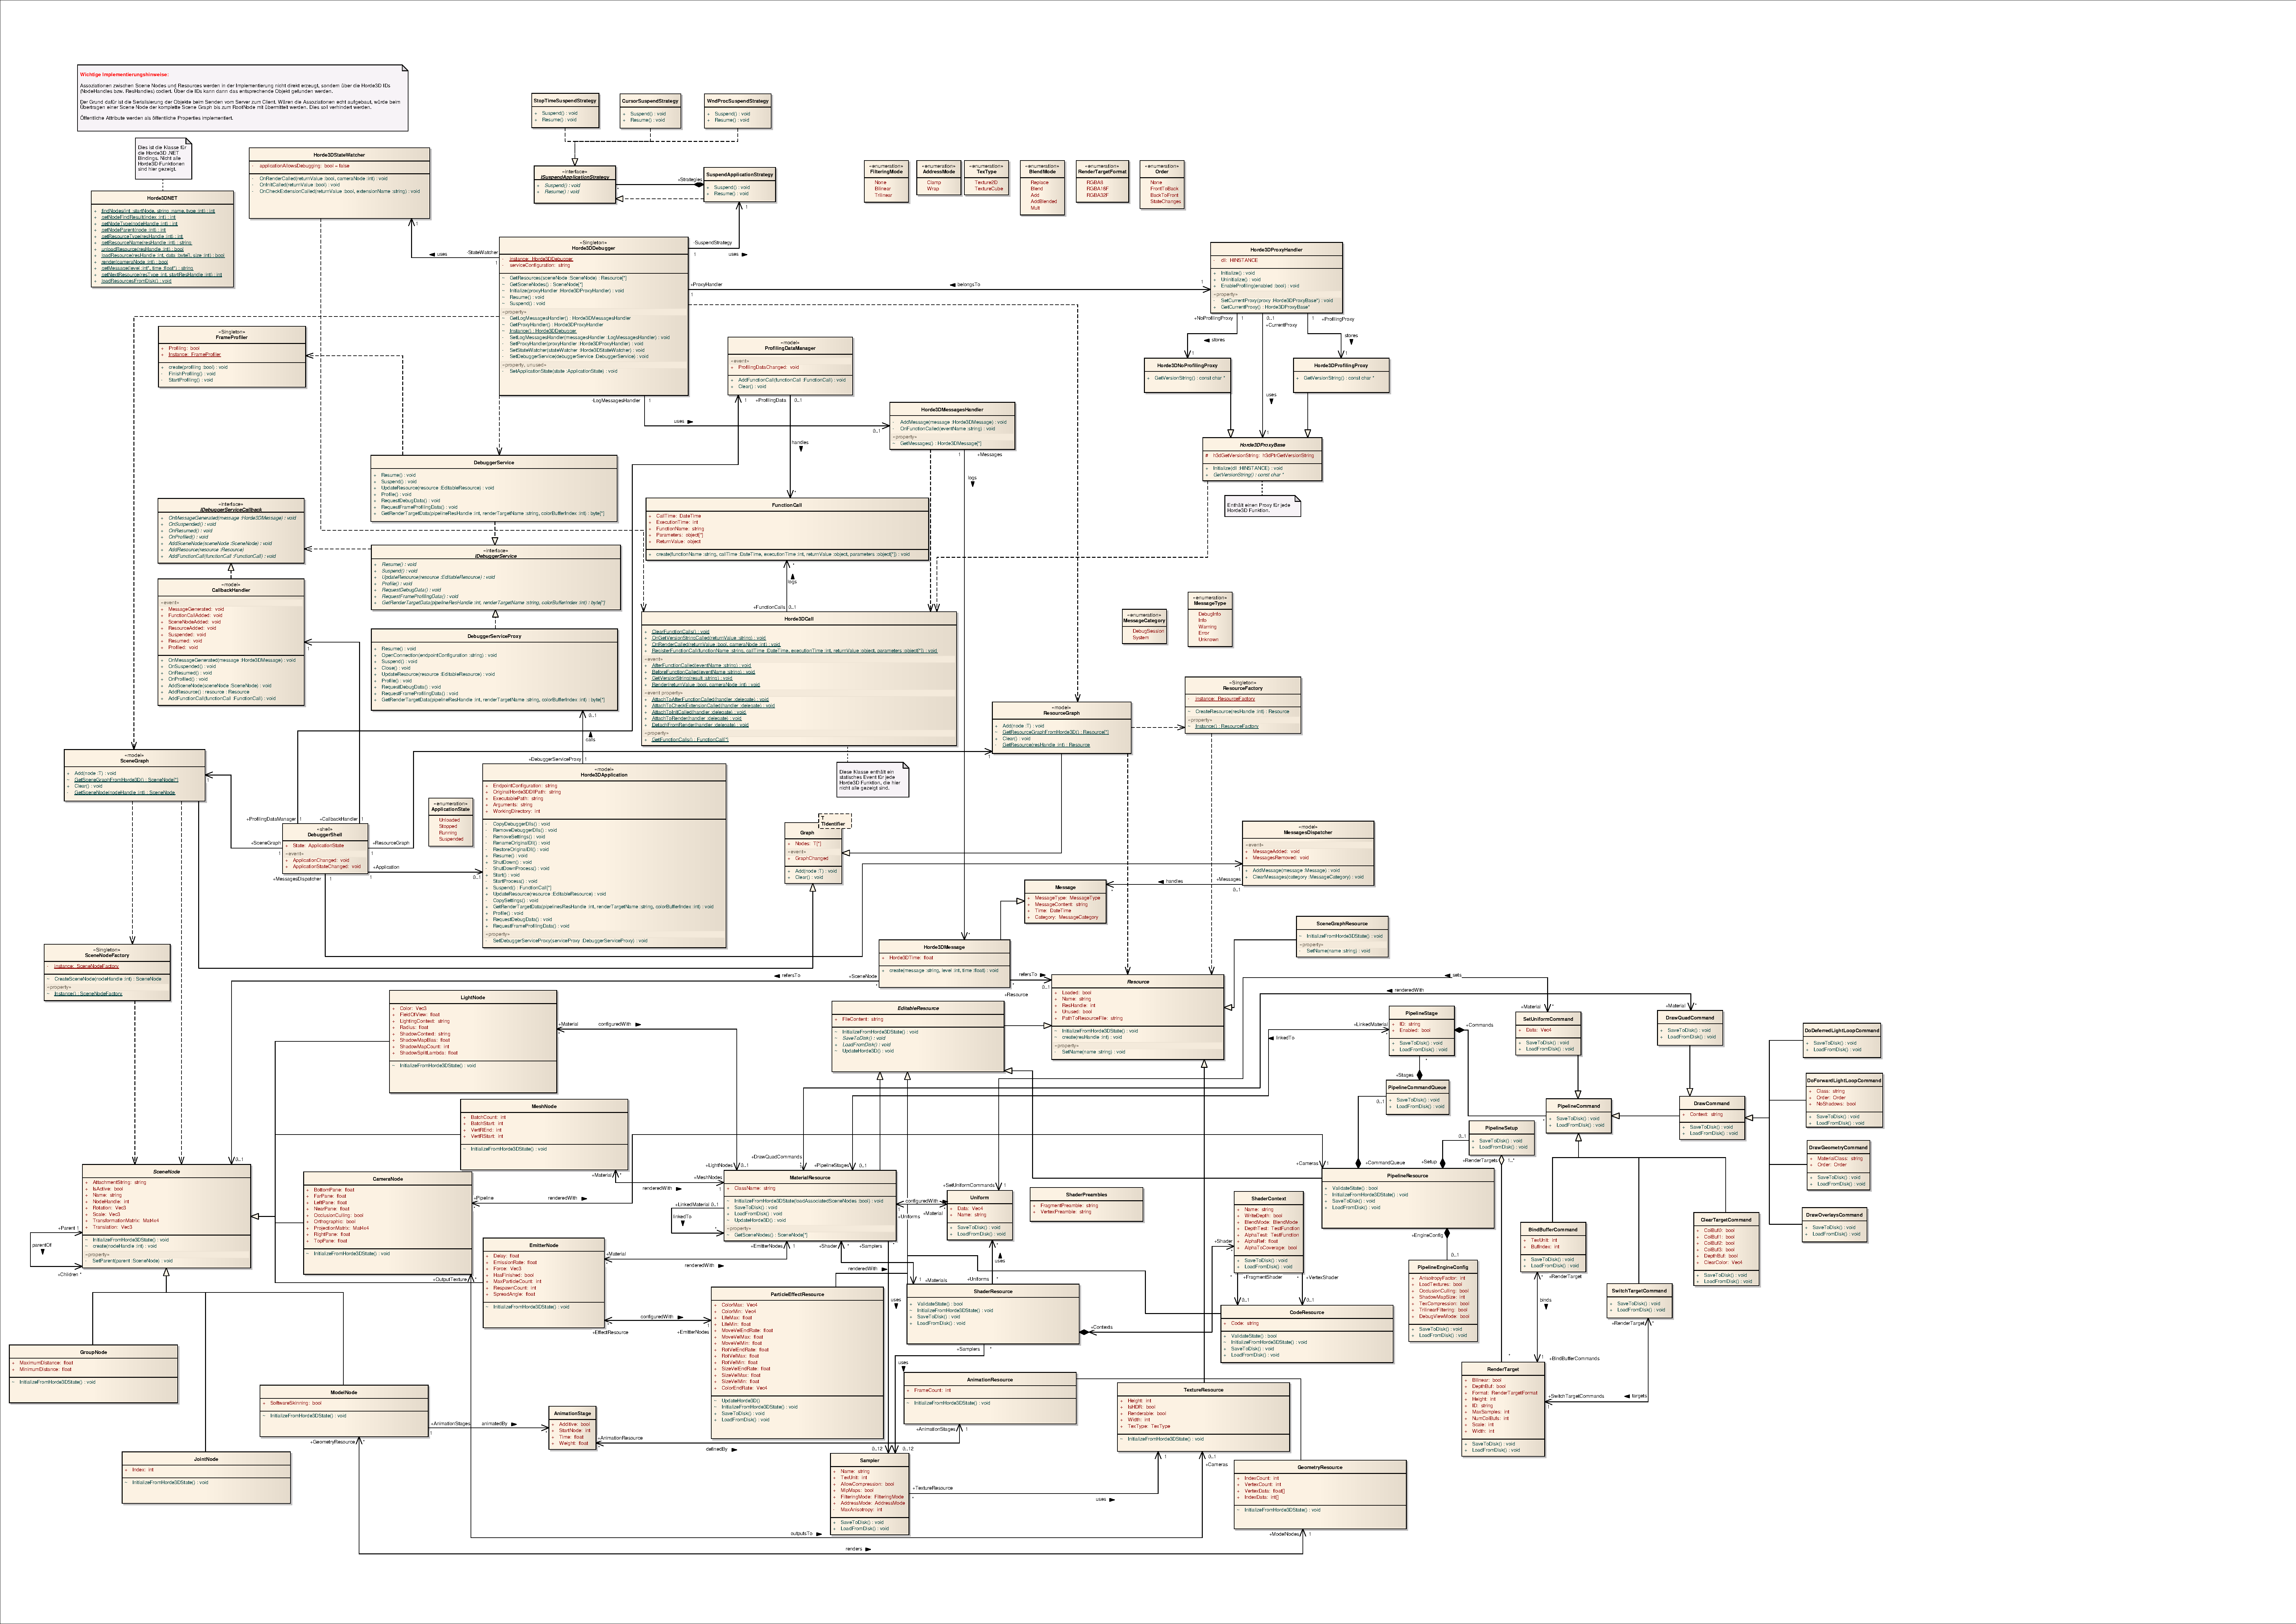
\includegraphics[trim = 70mm 468mm 865mm 230mm, clip, angle = 90, scale=0.7]{images/Designmodell.pdf}
\caption{Ausschnitt aus dem Designmodell f�r die Client-Server-Schnittstelle}\label{fig:clientServerInterfaceDesign}
\end{figure}

\begin{figure}[htp]
\centering
%trim=l b r t  	This option will crop the imported image by l from the left, b from the bottom, r from the right, and t  from the top. Where l, b, r and t are lengths. 
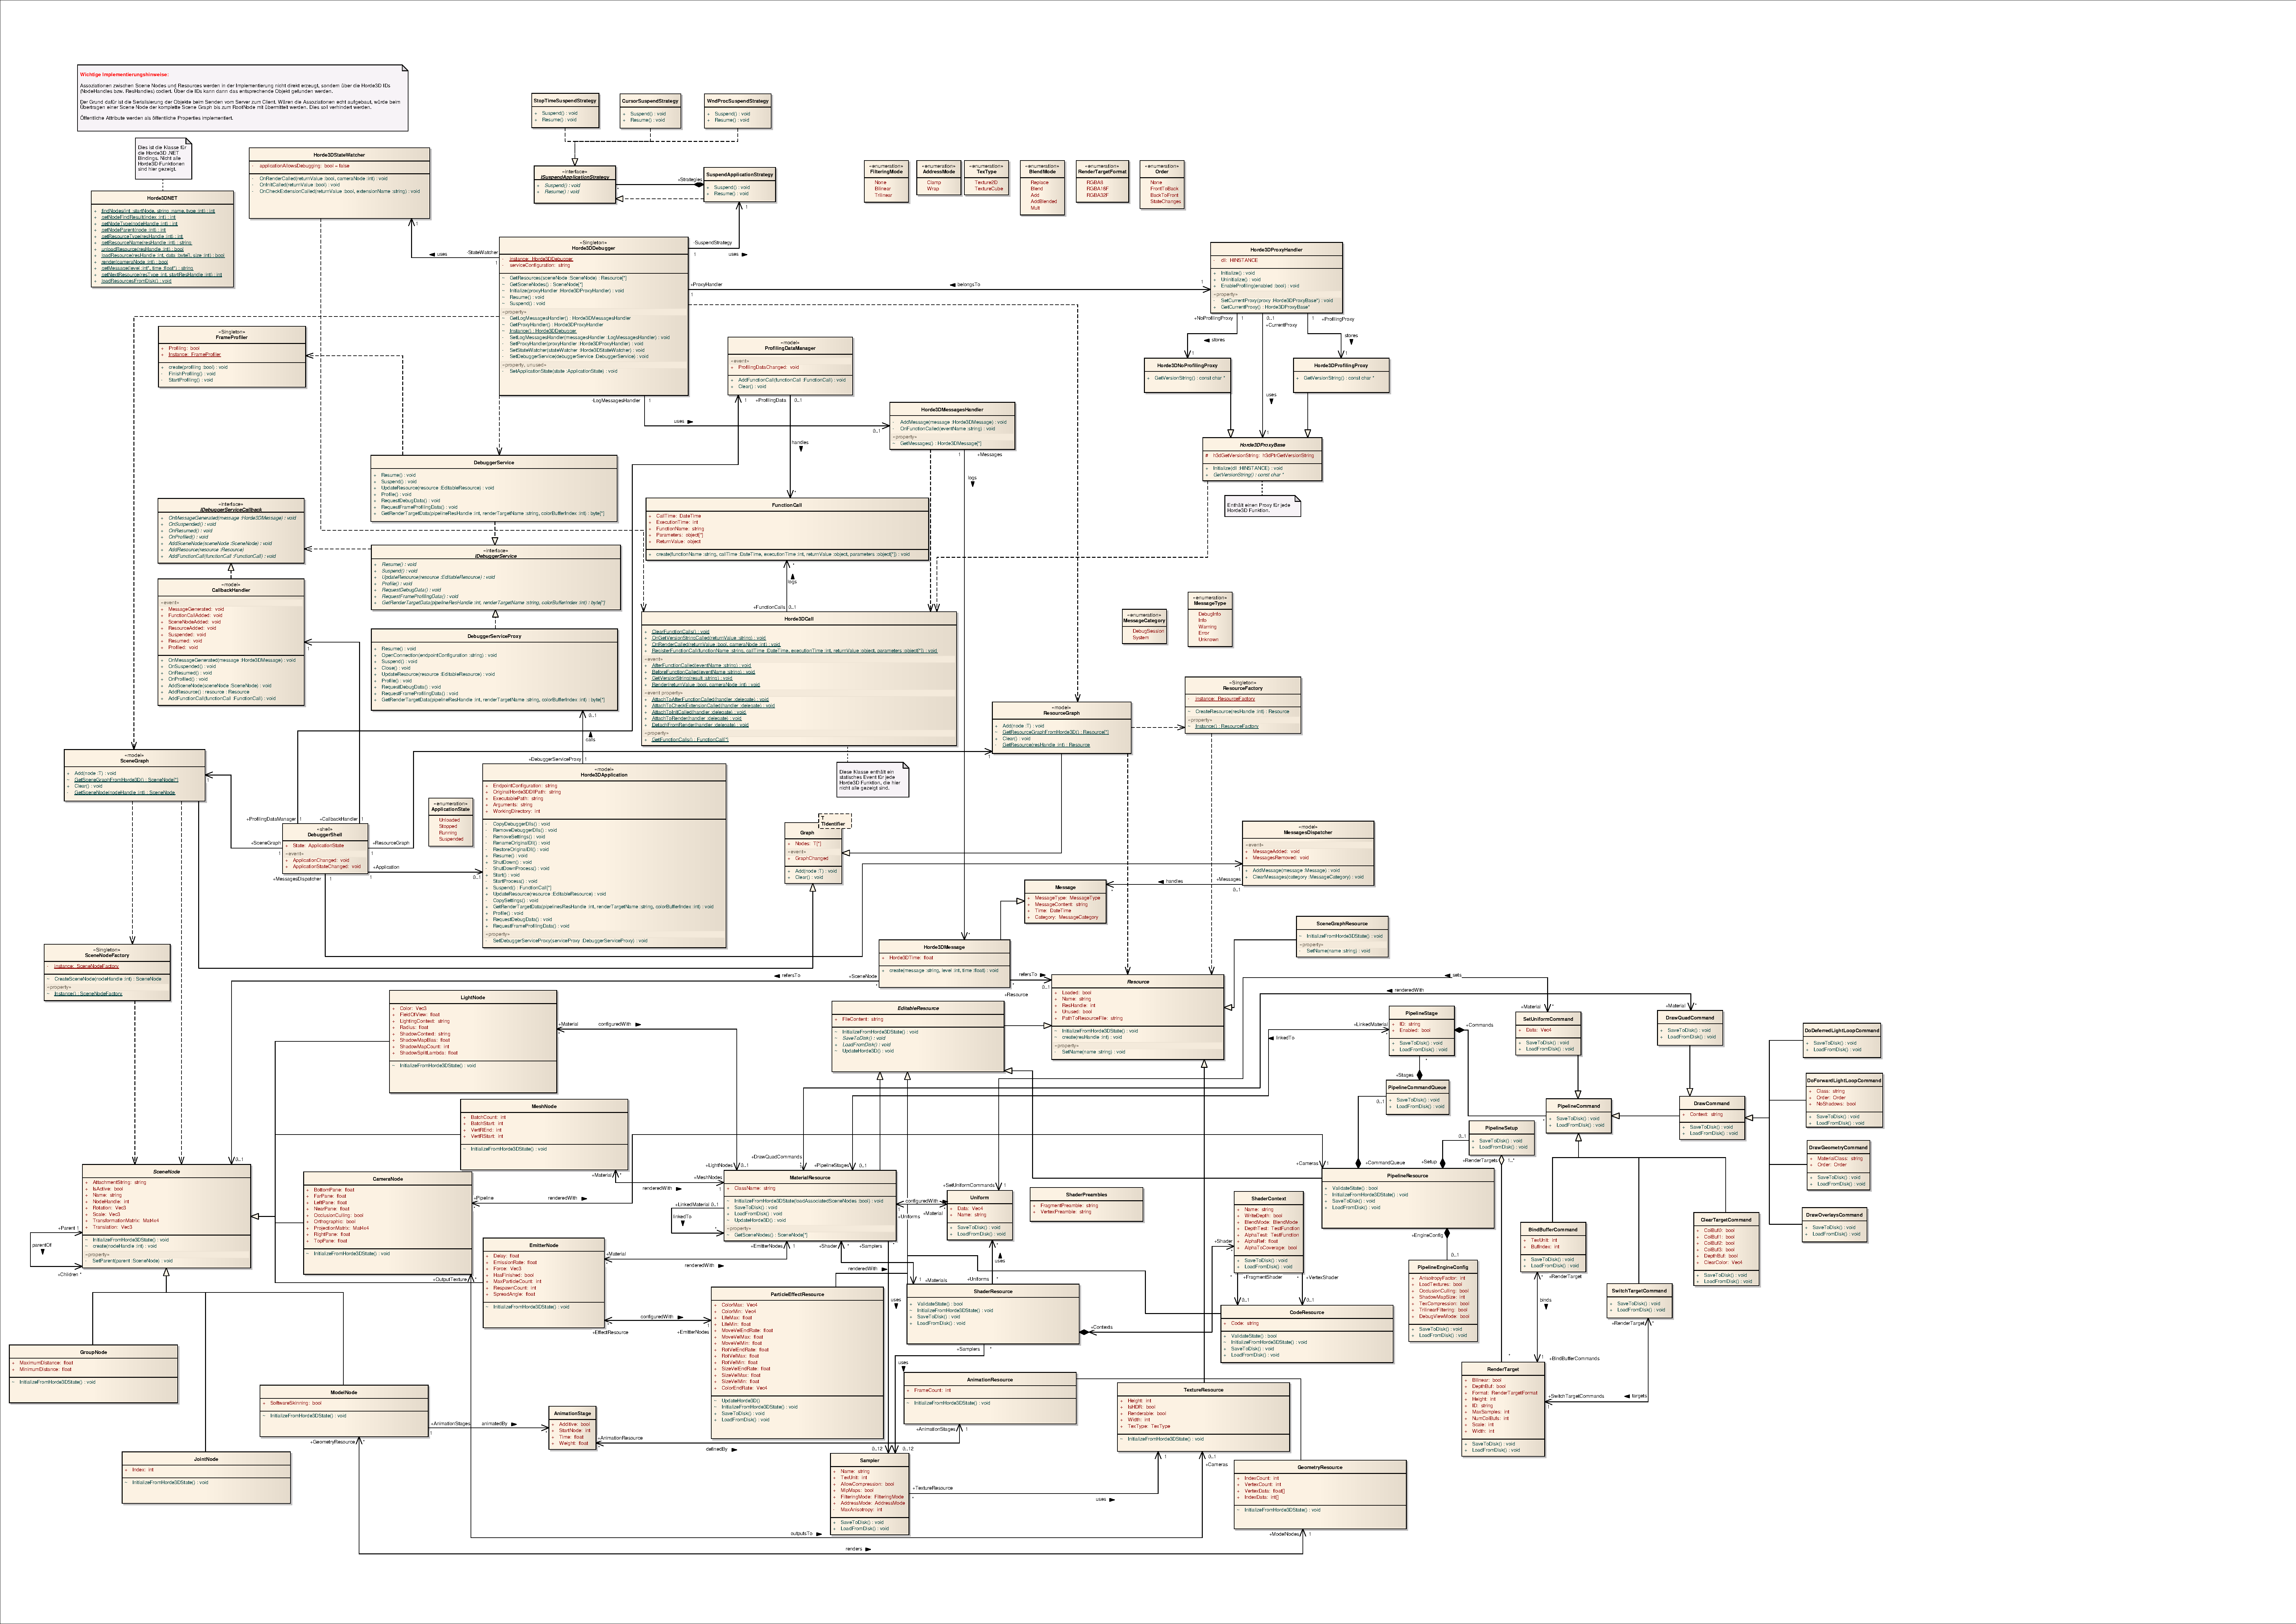
\includegraphics[trim = 250mm 725mm 760mm 40mm, clip, scale=0.7]{images/Designmodell.pdf}
\caption{Ausschnitt aus dem  Designklassen-Diagramm f�r die Anwendung des \emph{Strategy Patterns} zum Anhalten der Anwendung}\label{fig:suspendStrategyDesign}
\end{figure}

\begin{figure}[htp]
\centering
%trim=l b r t  	This option will crop the imported image by l from the left, b from the bottom, r from the right, and t  from the top. Where l, b, r and t are lengths. 
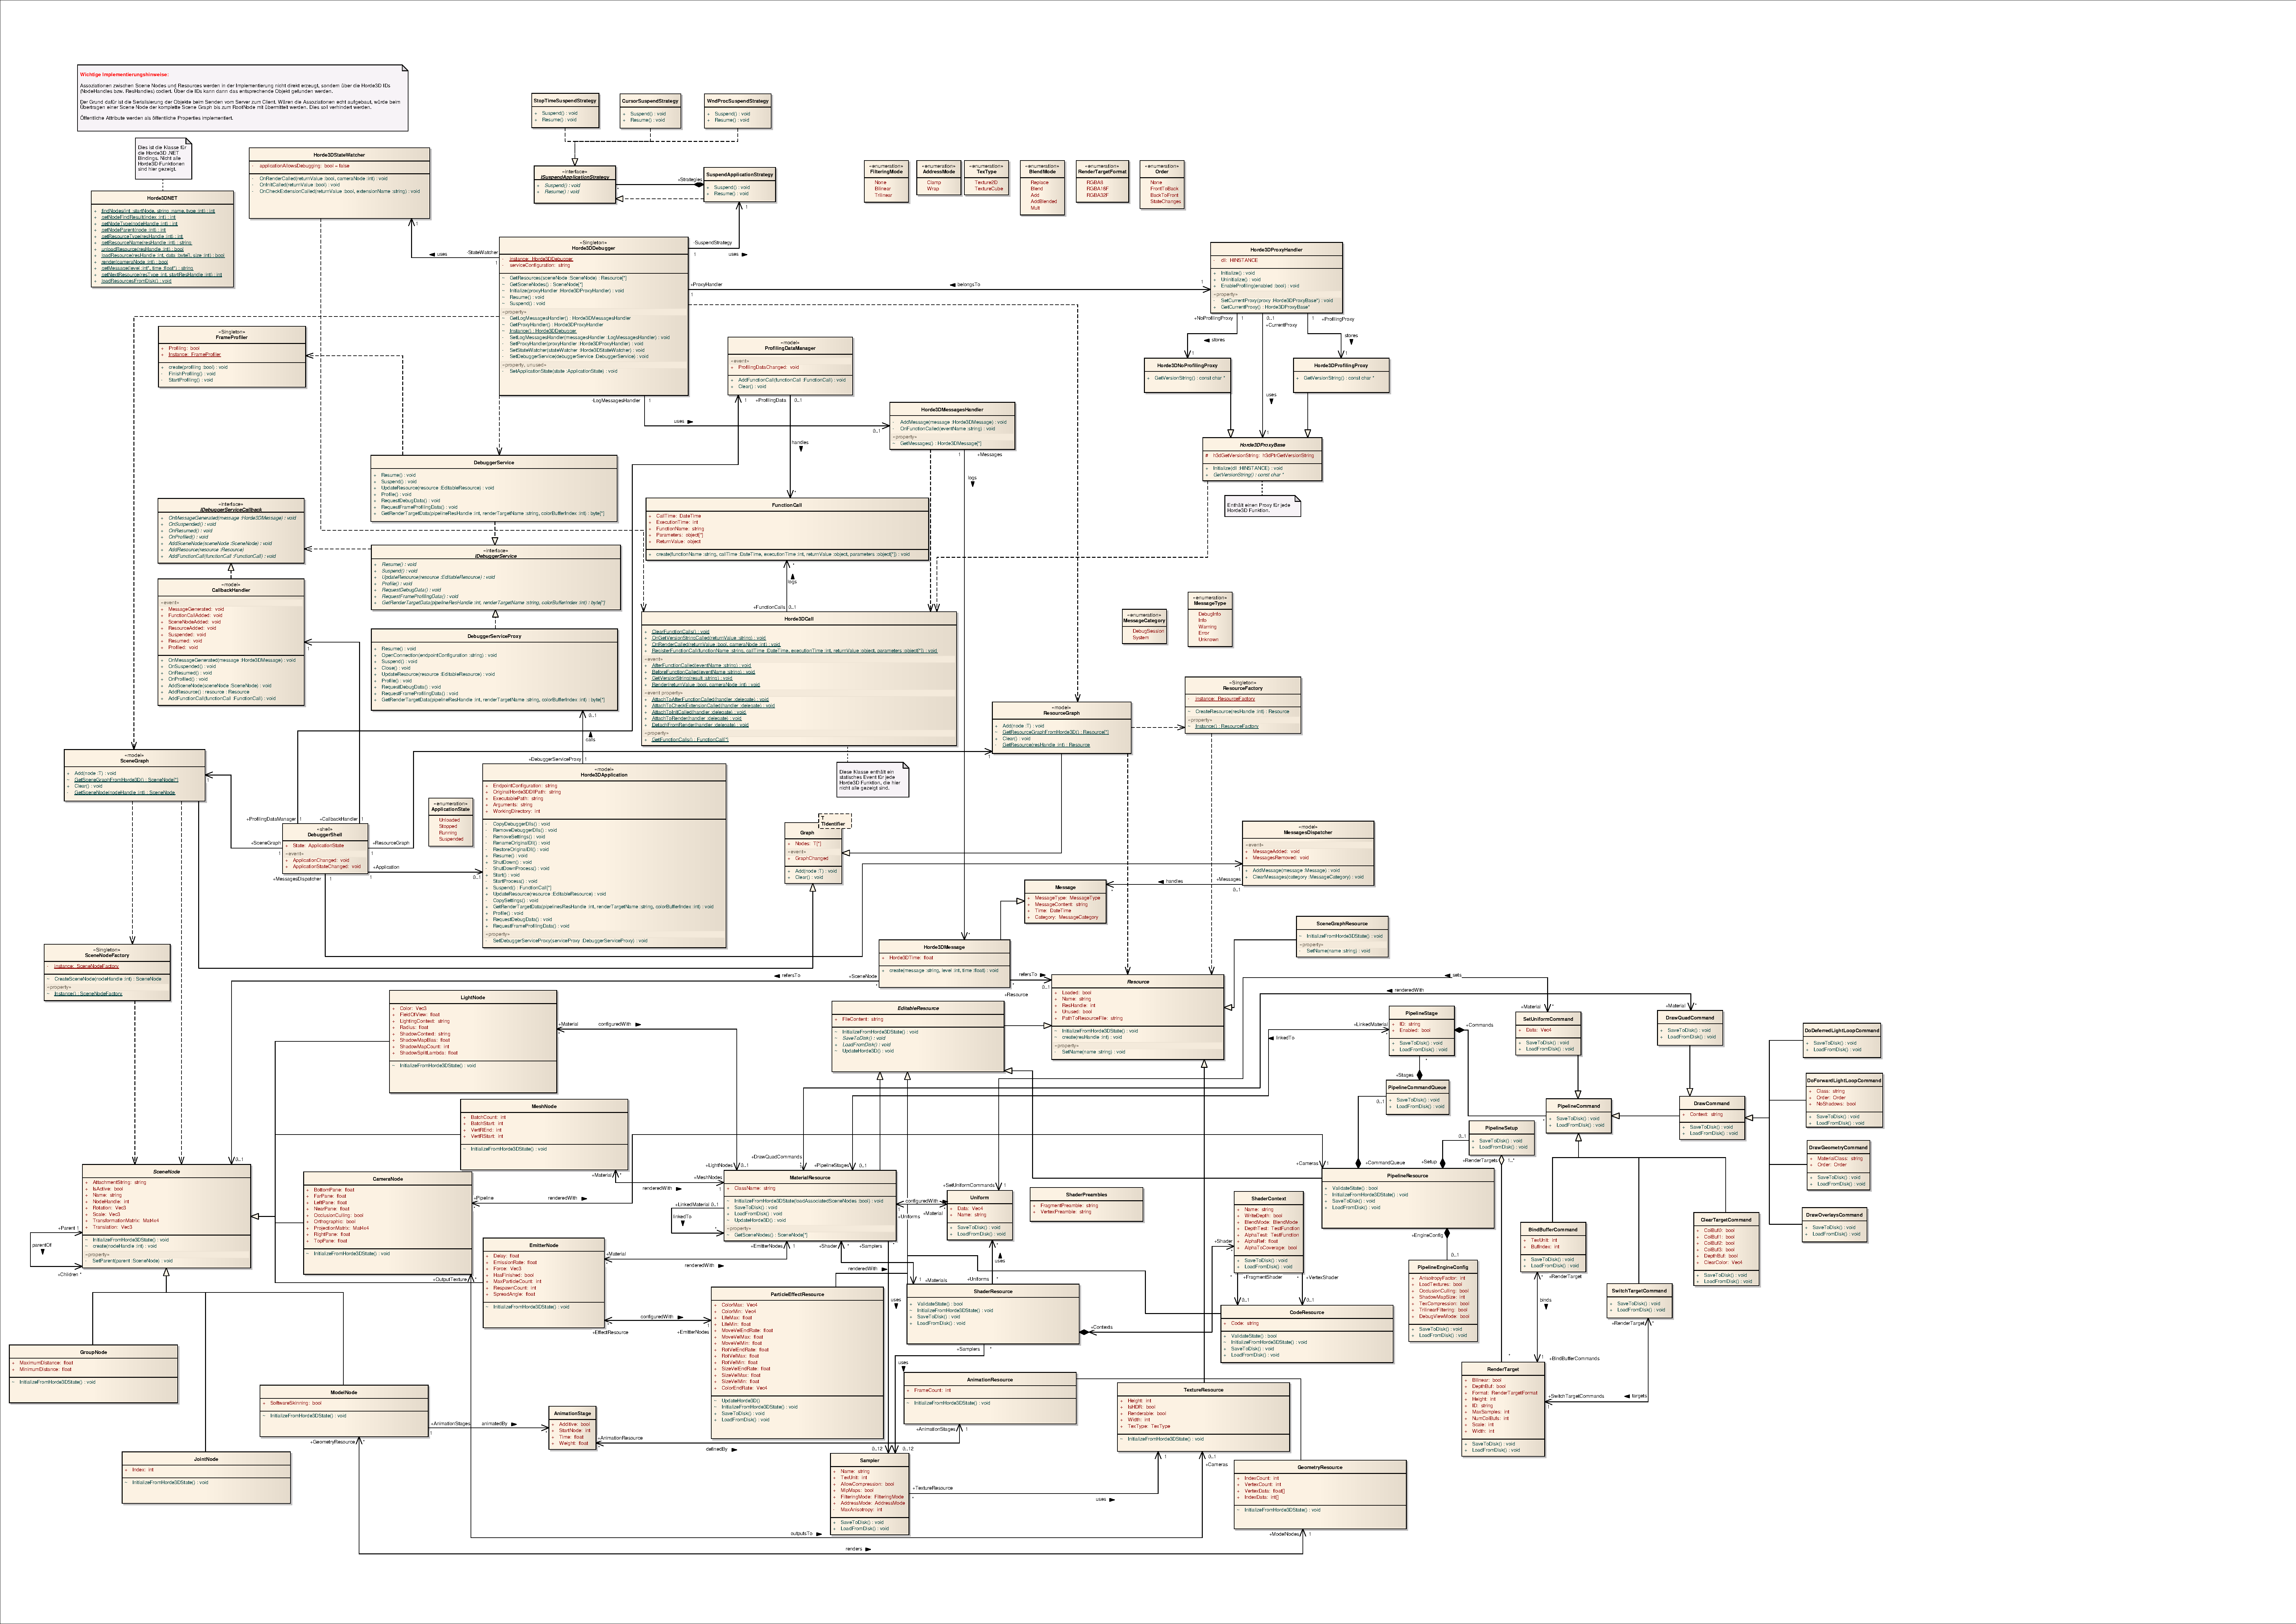
\includegraphics[trim = 585mm 570mm 450mm 125mm, clip, scale=0.7]{images/Designmodell.pdf}
\caption{Ausschnitt aus dem  Designklassen-Diagramm f�r die \Horde-\emph{Proxies}}\label{fig:proxyDesign}
\end{figure}

\begin{figure}[htp]
\centering
%trim=l b r t  	This option will crop the imported image by l from the left, b from the bottom, r from the right, and t  from the top. Where l, b, r and t are lengths. 
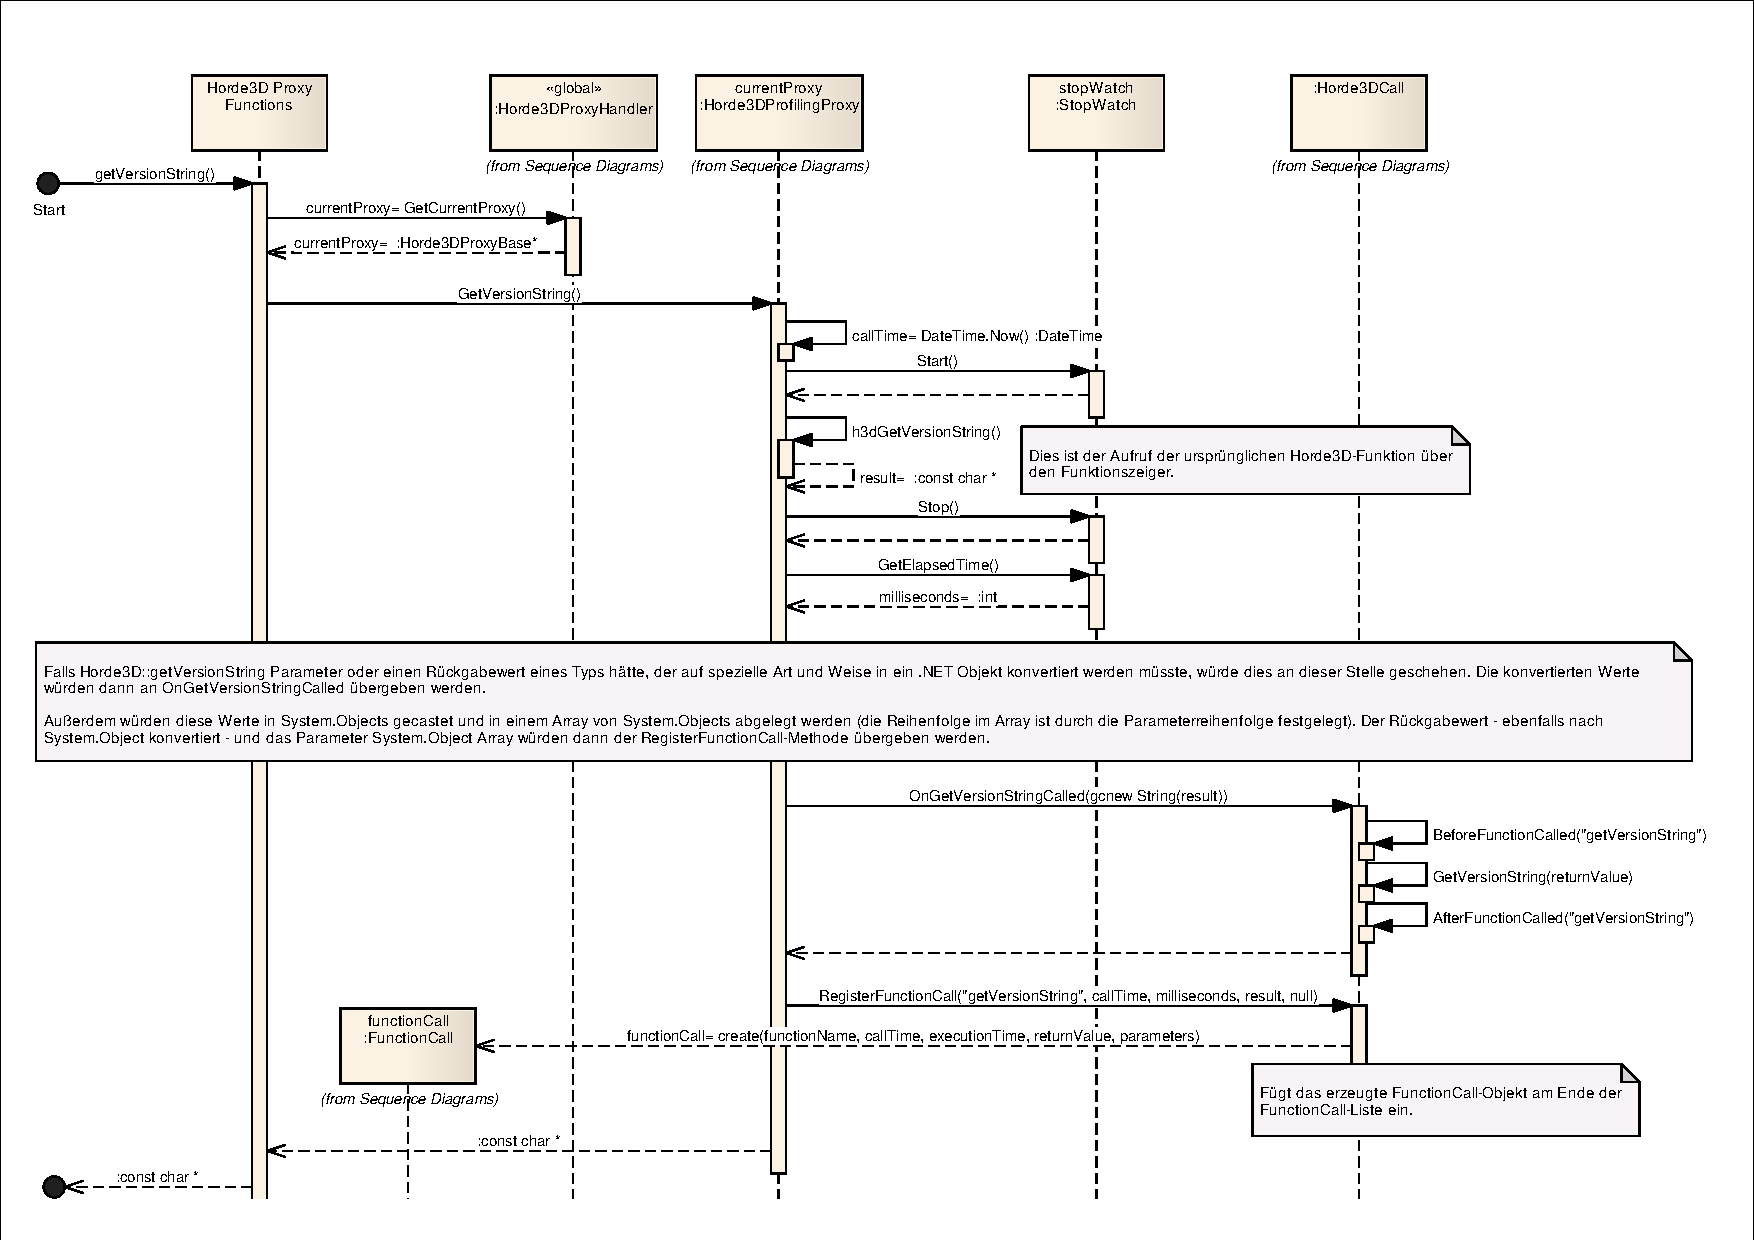
\includegraphics[trim = 5mm 1mm 1mm 5mm, clip, angle = 90, scale=0.7]{images/ProfilingProxySeq.pdf}
\caption{Sequenzdiagramm f�r den Aufruf von \texttt{Horde3D::getVersionString} bei aktiviertem Profiling}\label{fig:proxySeq}
\end{figure}

\begin{figure}[htp]
\centering
%trim=l b r t  	This option will crop the imported image by l from the left, b from the bottom, r from the right, and t  from the top. Where l, b, r and t are lengths. 
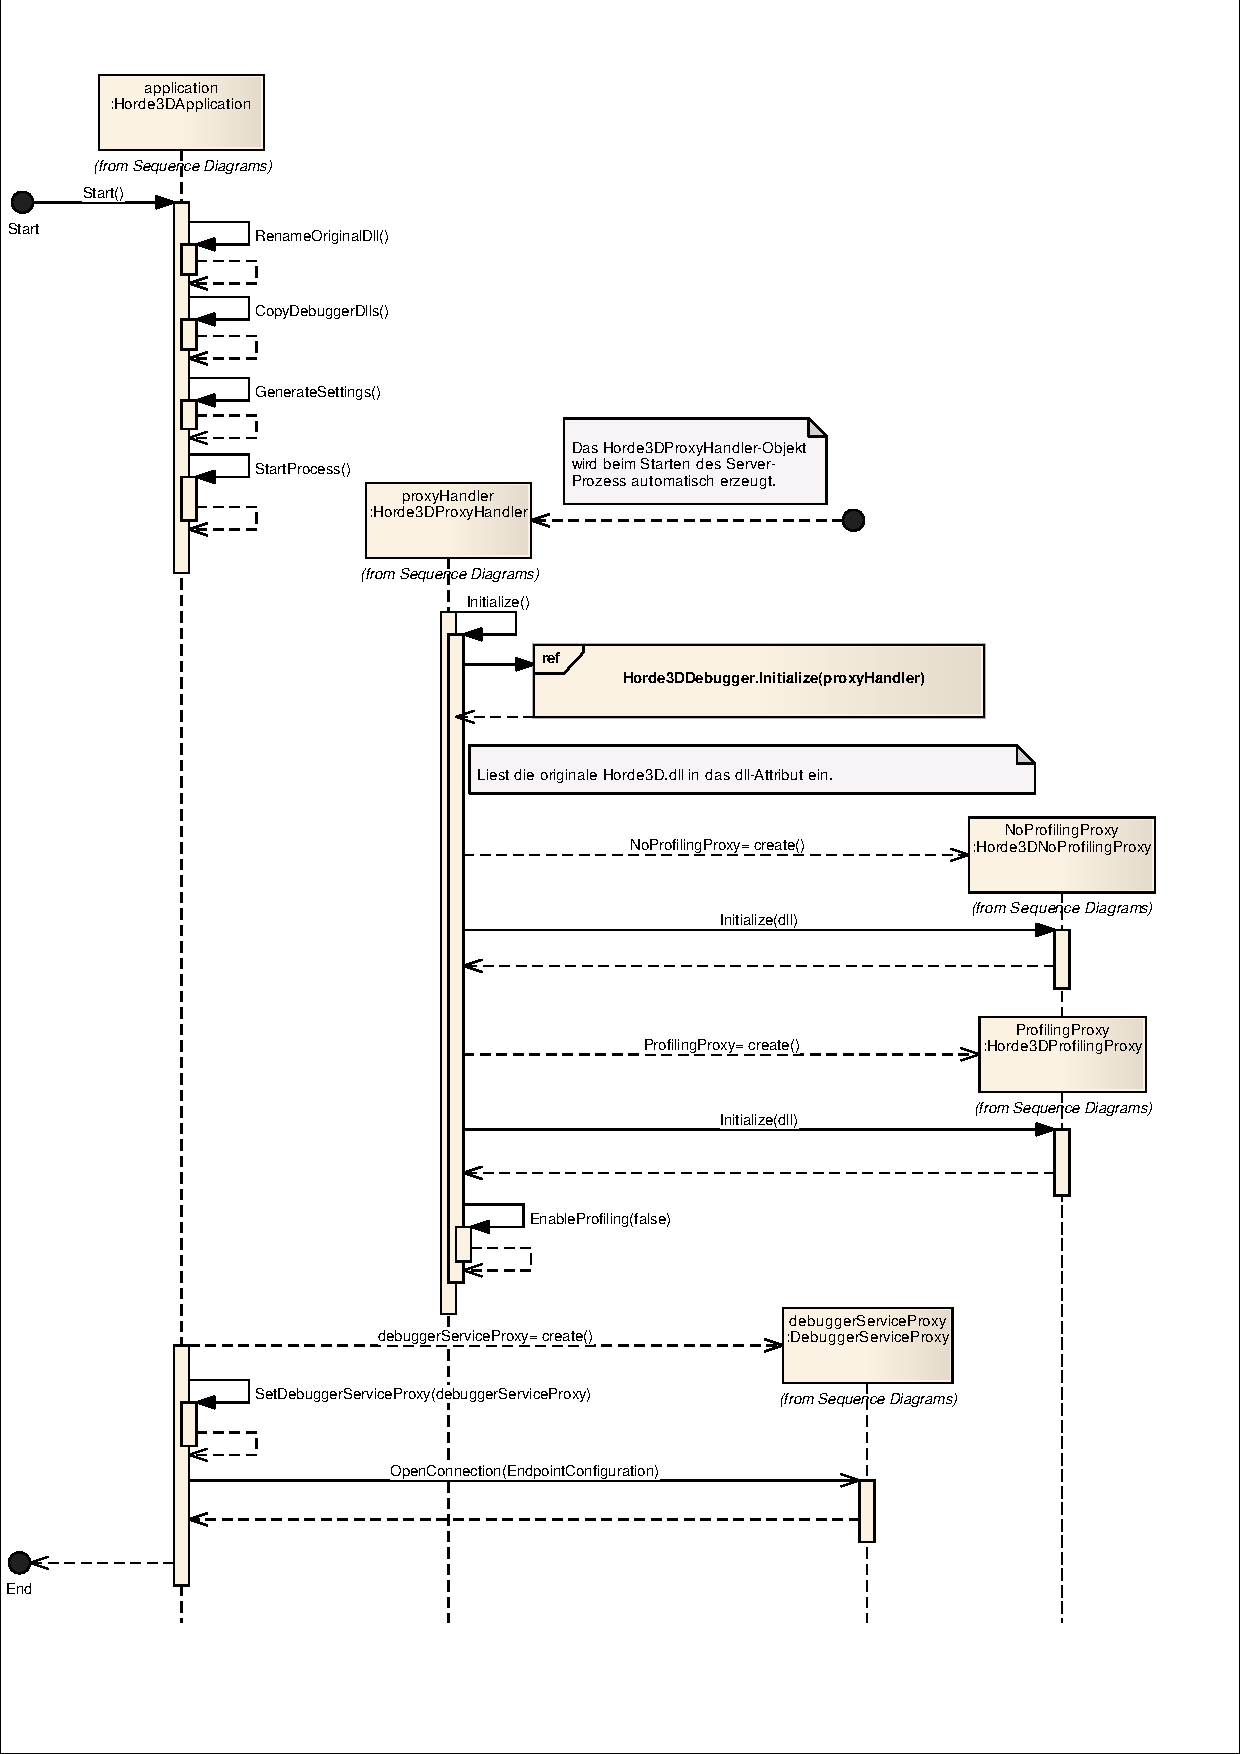
\includegraphics[trim = 1mm 20mm 10mm 5mm, clip, scale=0.7]{images/Horde3DApplication_Start.pdf}
\caption{Sequenzdiagramm f�r \texttt{Horde3DApplication.Start}}\label{fig:startSeq}
\end{figure}

\begin{figure}[htp]
\centering
%trim=l b r t  	This option will crop the imported image by l from the left, b from the bottom, r from the right, and t  from the top. Where l, b, r and t are lengths. 
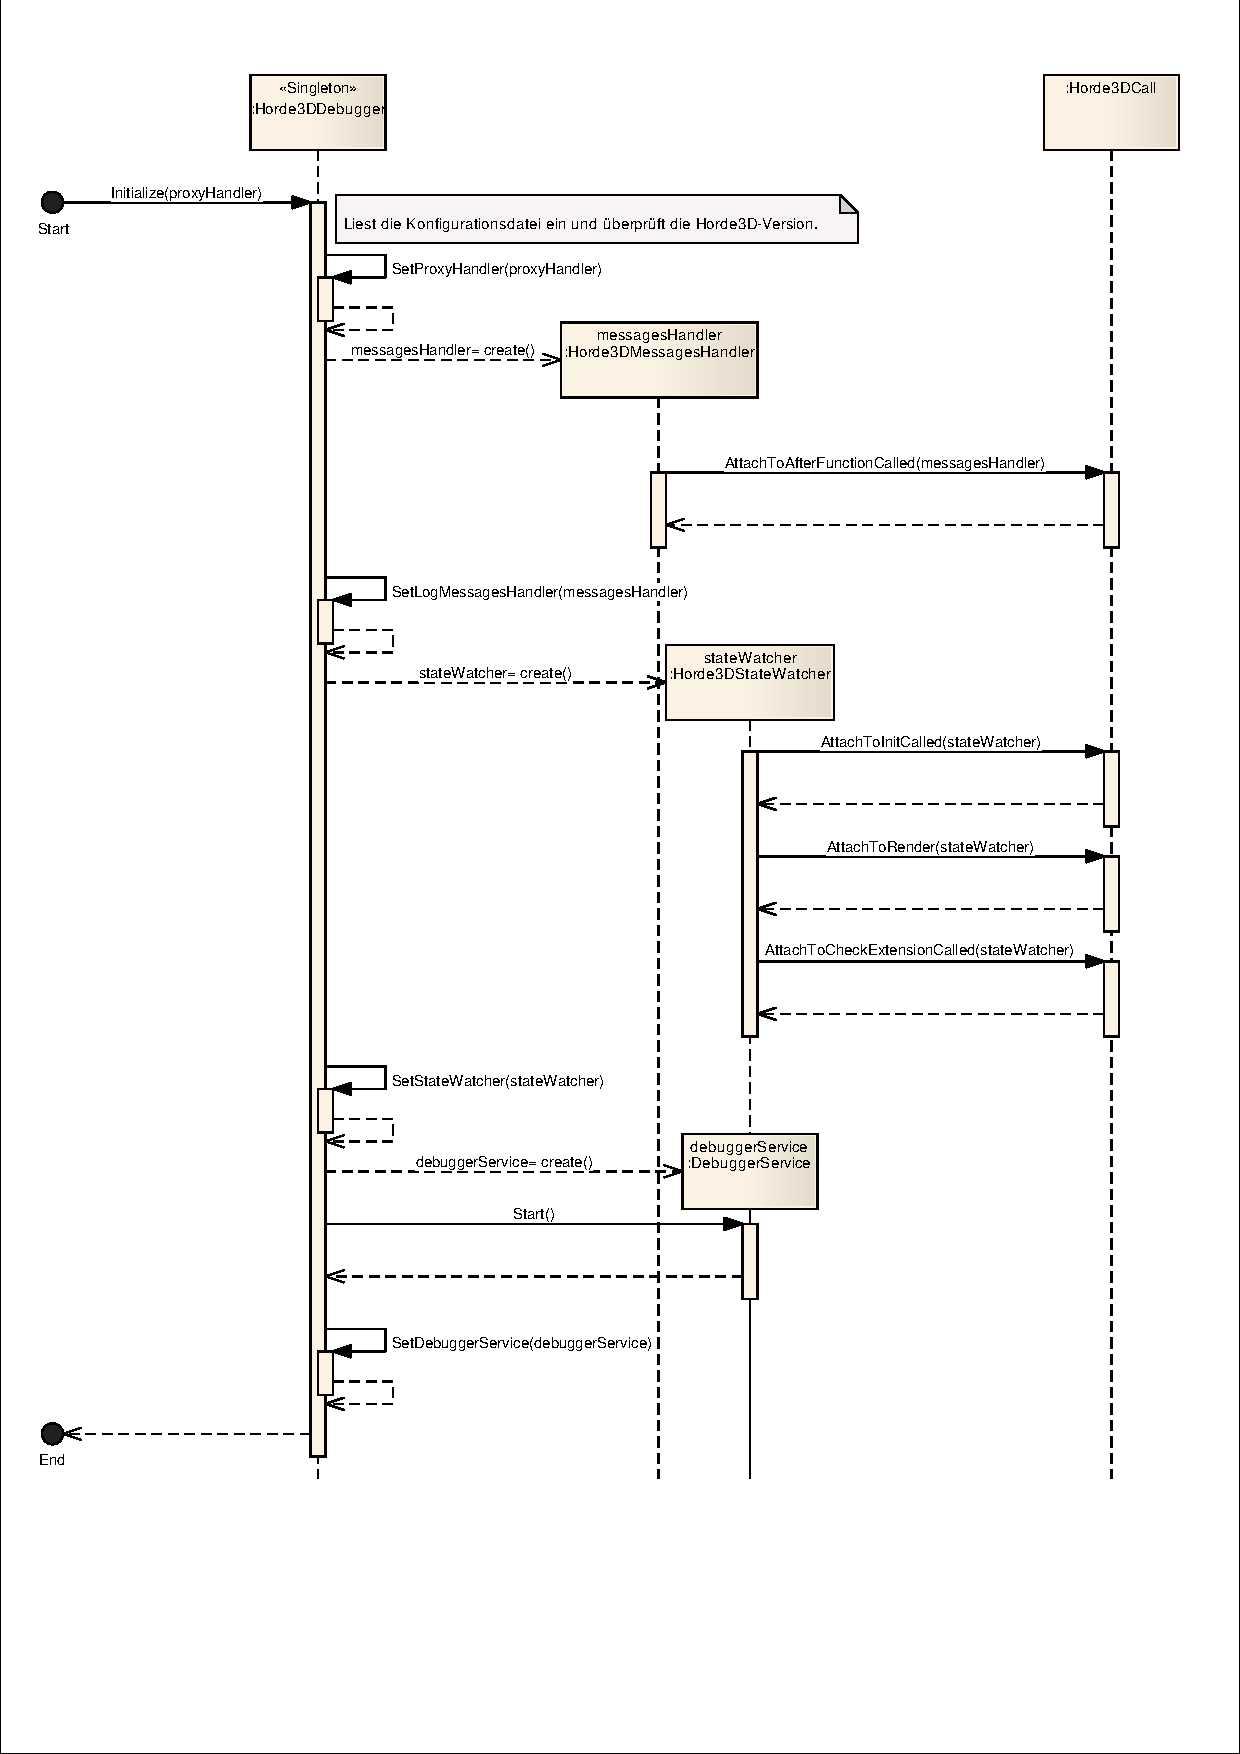
\includegraphics[trim = 5mm 45mm 5mm 5mm, clip, scale=0.7]{images/Horde3DDebugger_Initialize.pdf}
\caption{Sequenzdiagramm f�r \texttt{Horde3DDebugger.Initialize}}\label{fig:DebuggerInitSeq}
\end{figure}

\begin{figure}[htp]
\centering
%trim=l b r t  	This option will crop the imported image by l from the left, b from the bottom, r from the right, and t  from the top. Where l, b, r and t are lengths. 
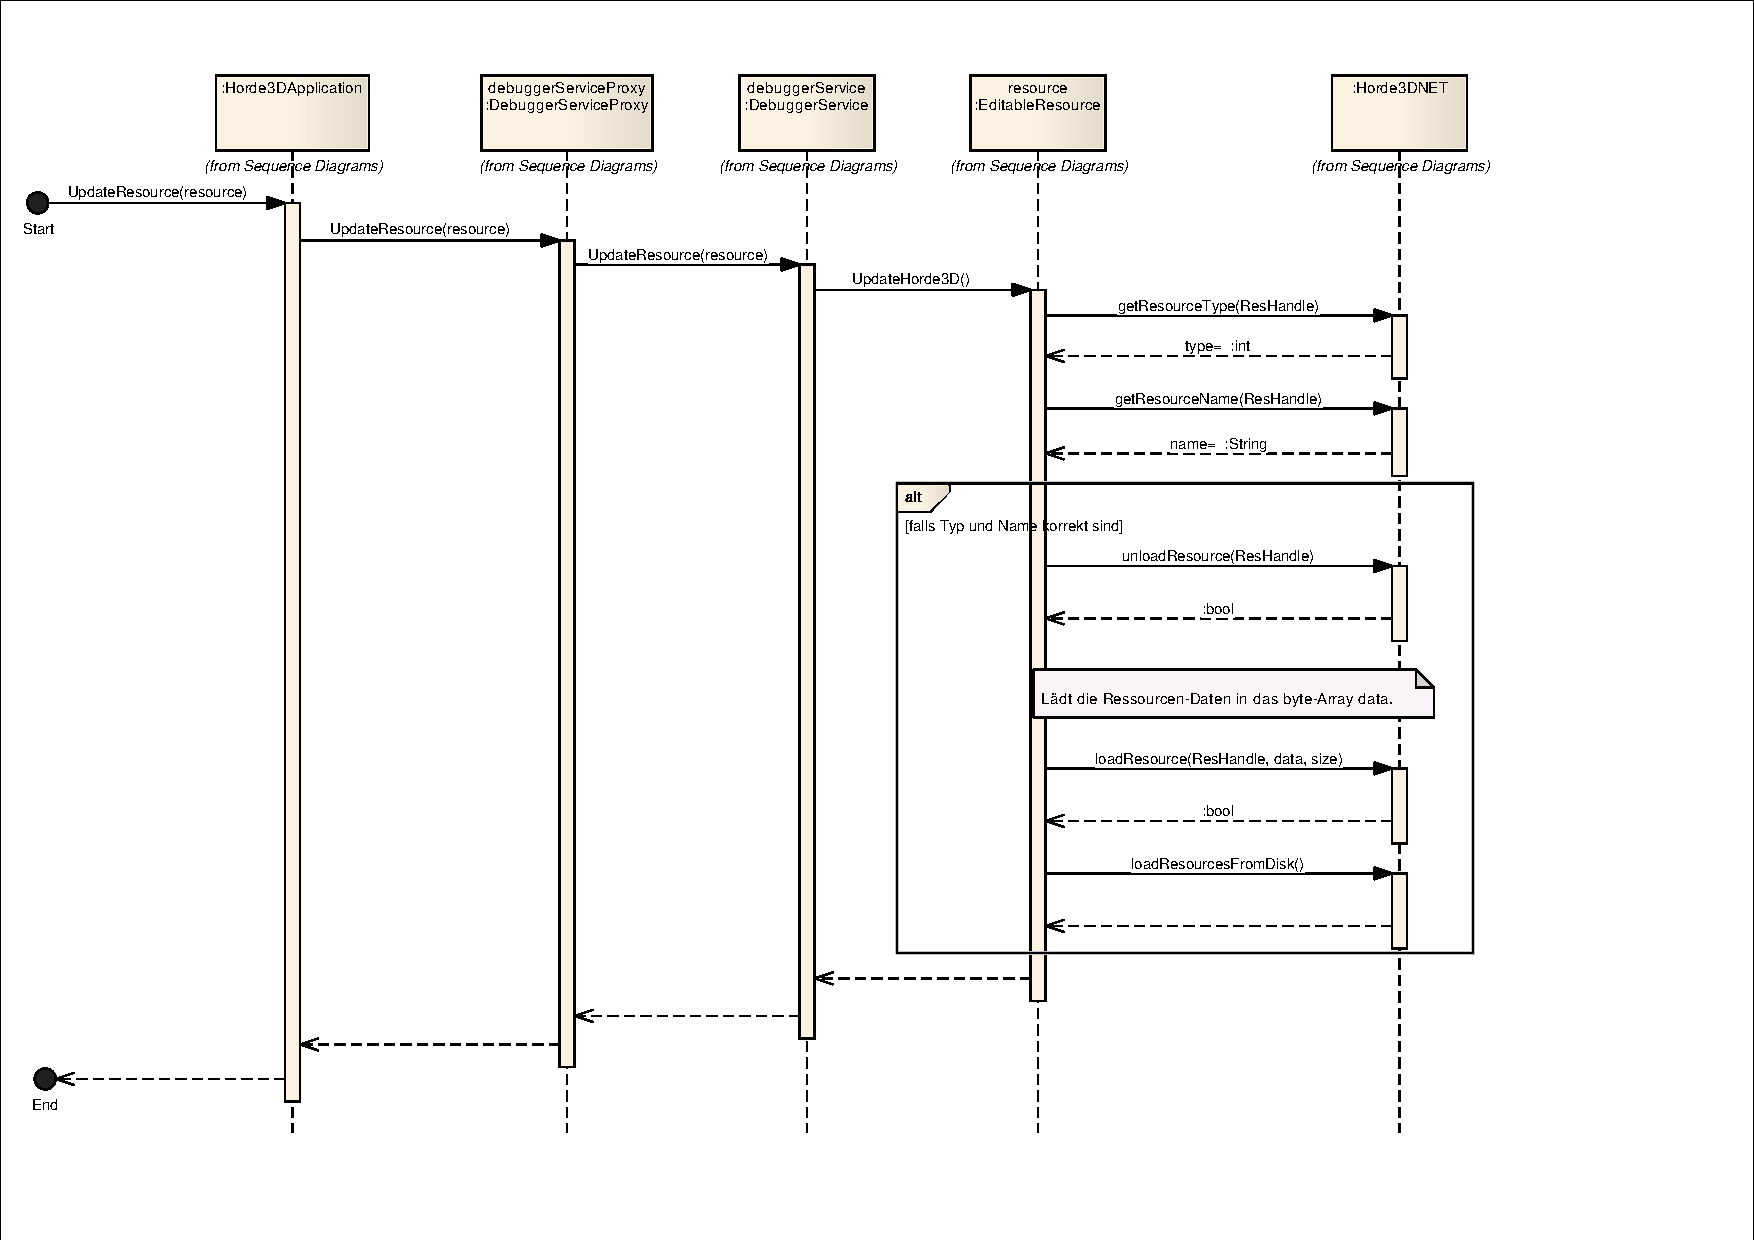
\includegraphics[trim = 1mm 15mm 5mm 5mm, clip, angle = 90, scale=0.7]{images/UpdateResource.pdf}
\caption{Sequenzdiagramm f�r \texttt{Horde3DApplication.UpdateResource}}\label{fig:UpdateResourceSeq}
\end{figure}

\begin{figure}[htp]
\centering
%trim=l b r t  	This option will crop the imported image by l from the left, b from the bottom, r from the right, and t  from the top. Where l, b, r and t are lengths. 
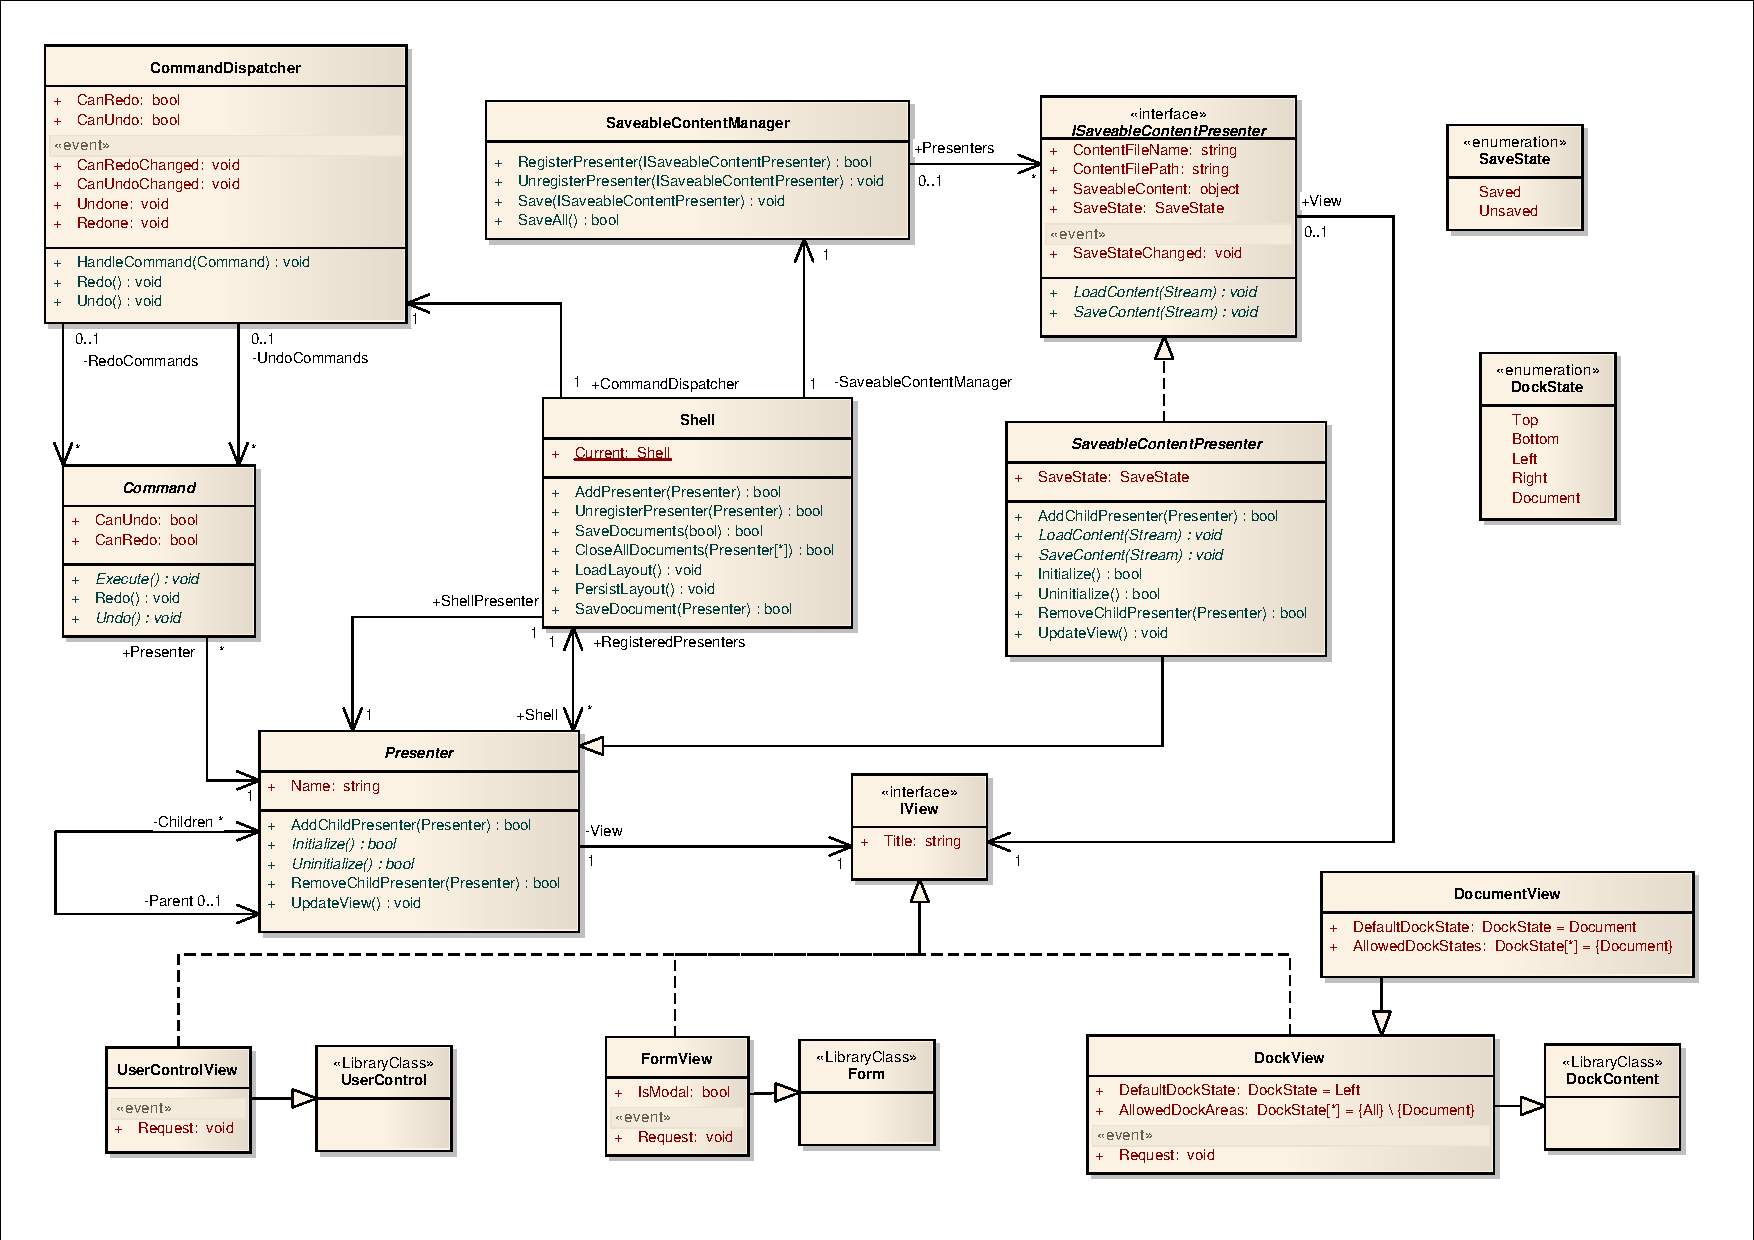
\includegraphics[trim = 5mm 5mm 5mm 5mm, clip, angle = 90, scale=0.7]{images/GuiClass.pdf}
\caption{Designklassen-Diagramm f�r das GUI-Framework}\label{fig:guiClass}
\end{figure}

\chapter{Artefakte der Implementierungs-Phase}

\begin{figure}[htp]
\centering
%trim=l b r t  	This option will crop the imported image by l from the left, b from the bottom, r from the right, and t  from the top. Where l, b, r and t are lengths. 
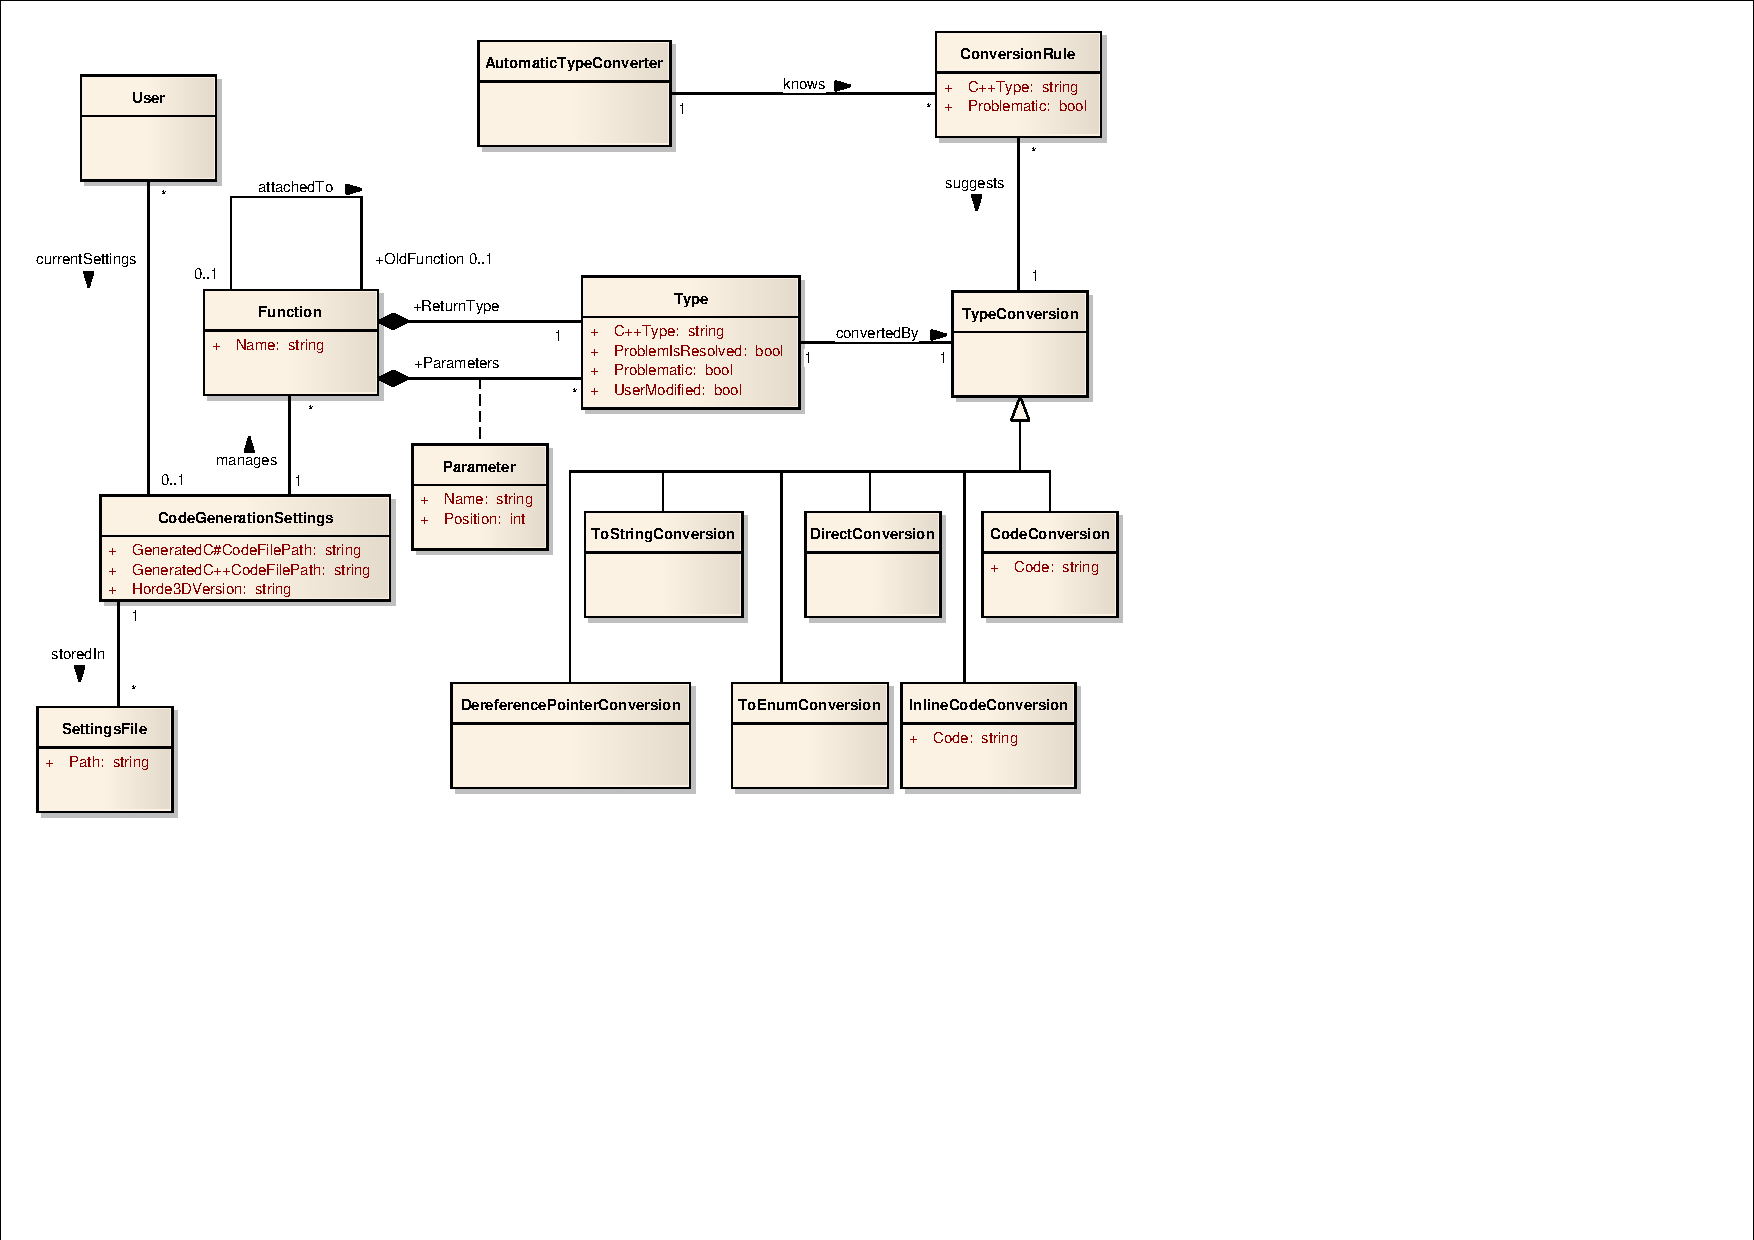
\includegraphics[trim = 5mm 70mm 85mm 5mm, clip, angle = 0, scale=0.7]{images/CodeGen_DomainModell.pdf}
\caption{Das Konzeptmodell des Code Generators}\label{fig:cgDomain}
\end{figure}

\begin{figure}[htp]
\centering
%trim=l b r t  	This option will crop the imported image by l from the left, b from the bottom, r from the right, and t  from the top. Where l, b, r and t are lengths. 
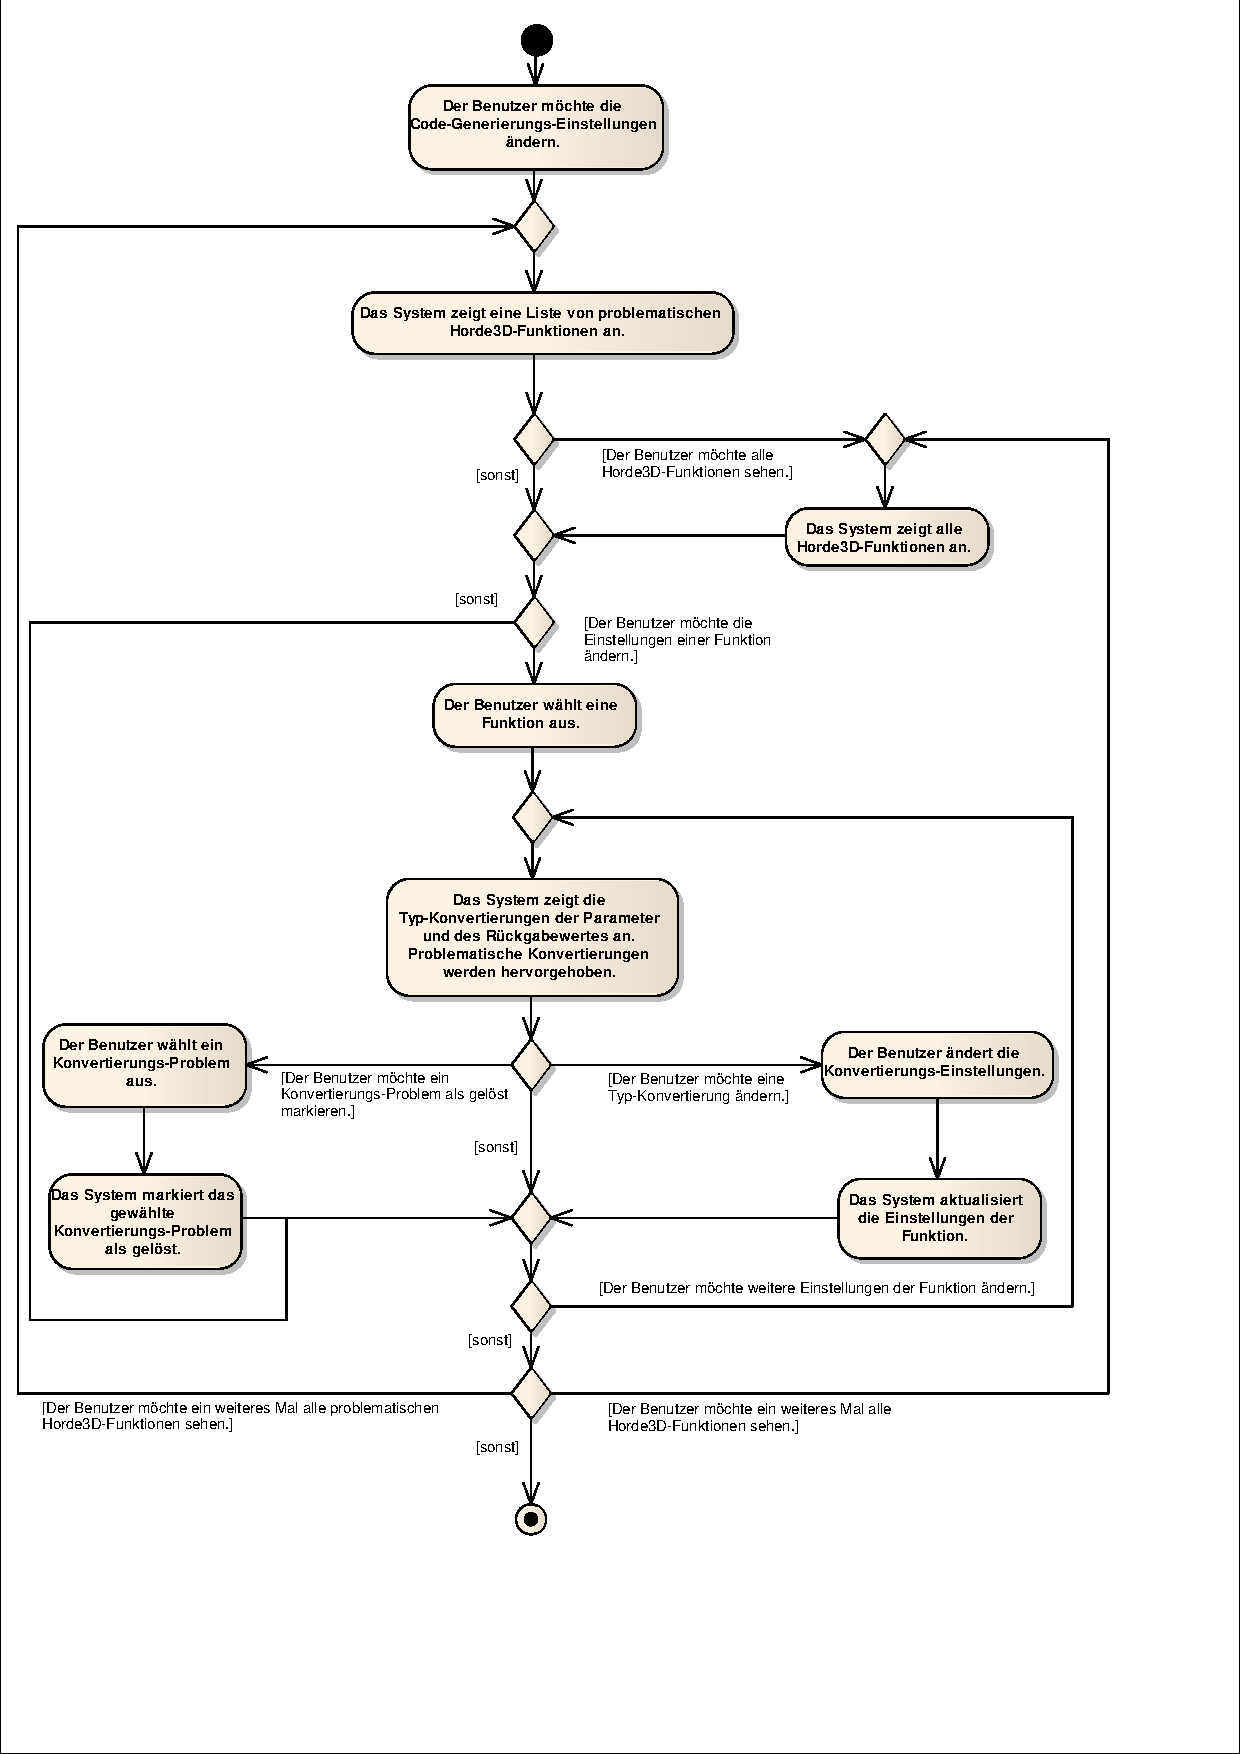
\includegraphics[trim = 1mm 30mm 20mm 1mm, clip, scale=0.7]{images/CodeGen_Change.pdf}
\caption{Aktivit�tsdiagramm f�r den Anwendungsfall "`�ndern der Einstellungen der Code-Generierung"'}\label{fig:cgChange}
\end{figure}

\begin{figure}[htp]
\centering
%trim=l b r t  	This option will crop the imported image by l from the left, b from the bottom, r from the right, and t  from the top. Where l, b, r and t are lengths. 
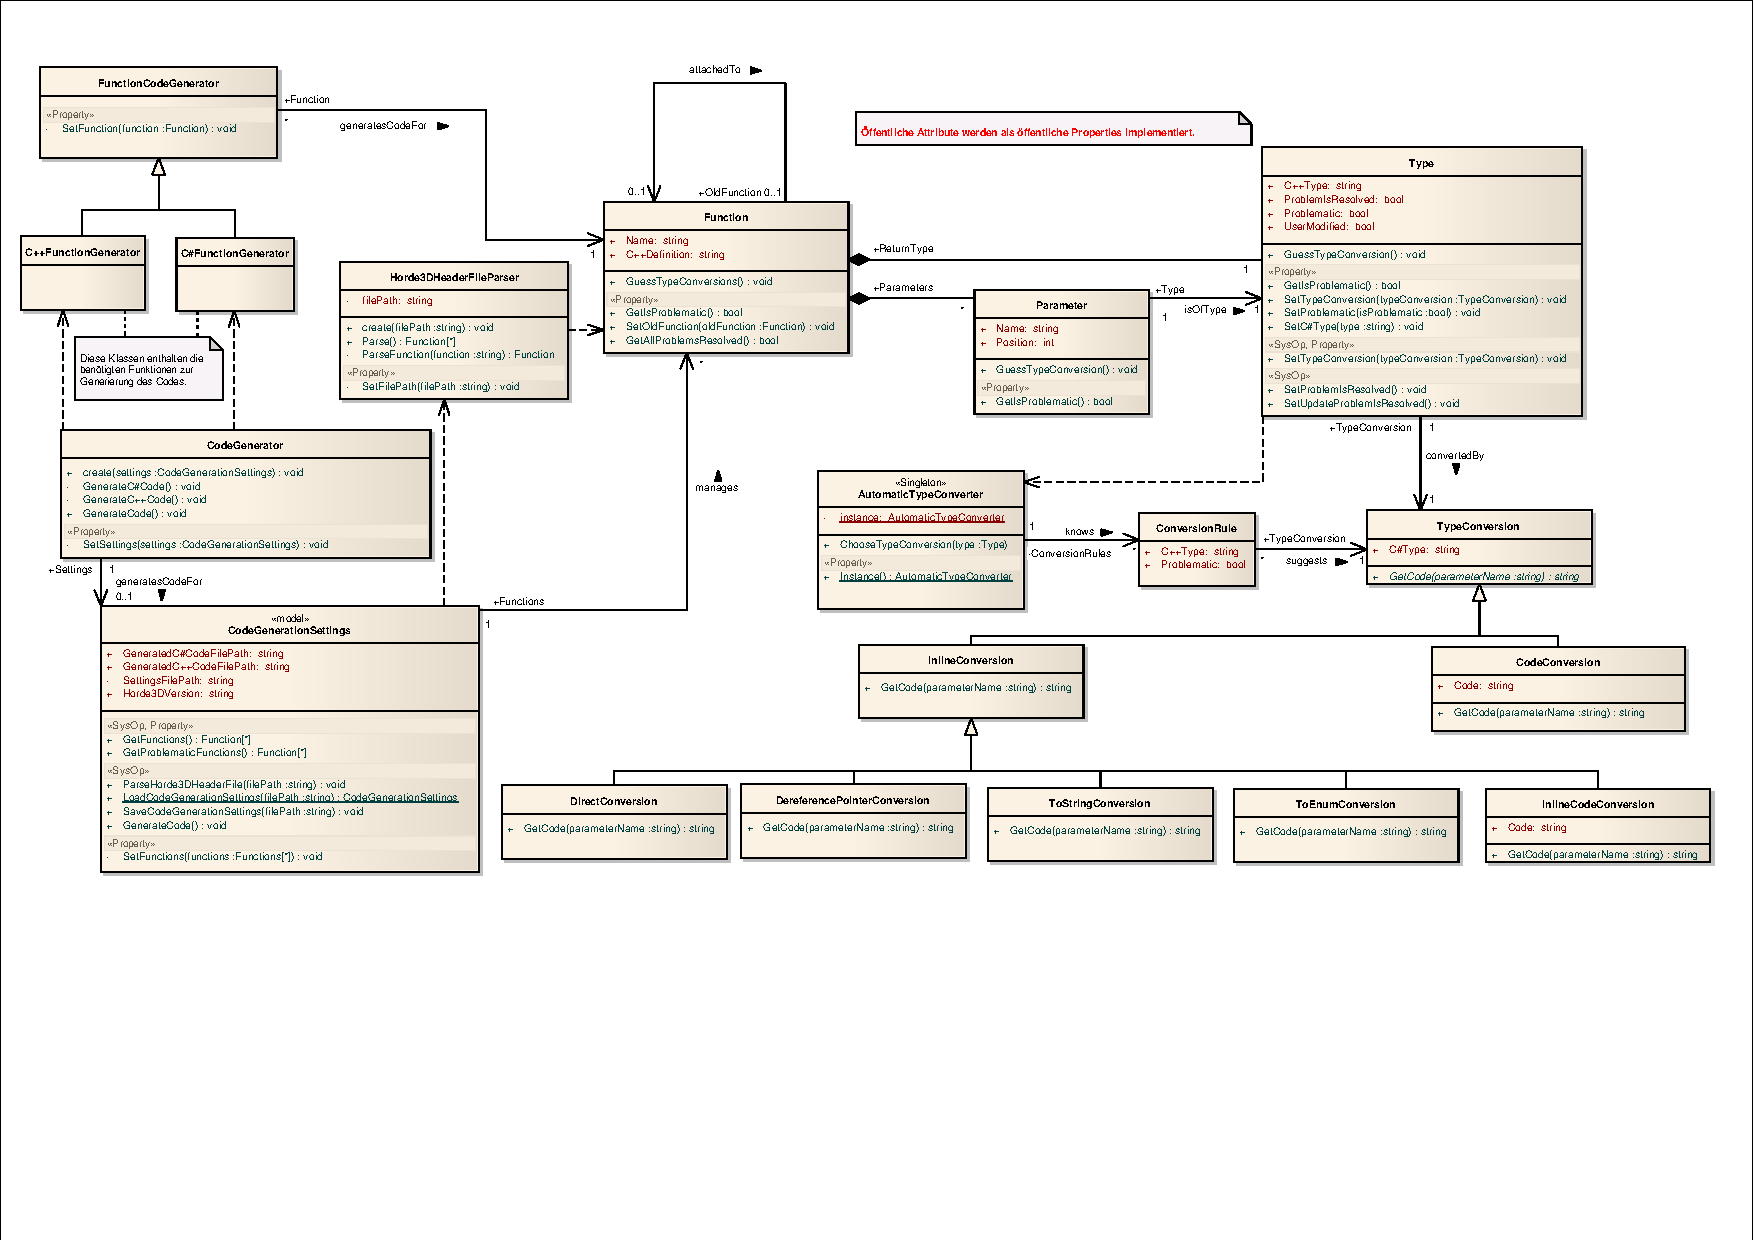
\includegraphics[trim = 1mm 30mm 1mm 1mm, angle = 90, clip, scale=0.7]{images/CodeGen_DesignModell.pdf}
\caption{Das Designmodell des Code Generators}\label{fig:cgDesign}
\end{figure}

\begin{figure}[htp]
\centering
%trim=l b r t  	This option will crop the imported image by l from the left, b from the bottom, r from the right, and t  from the top. Where l, b, r and t are lengths. 
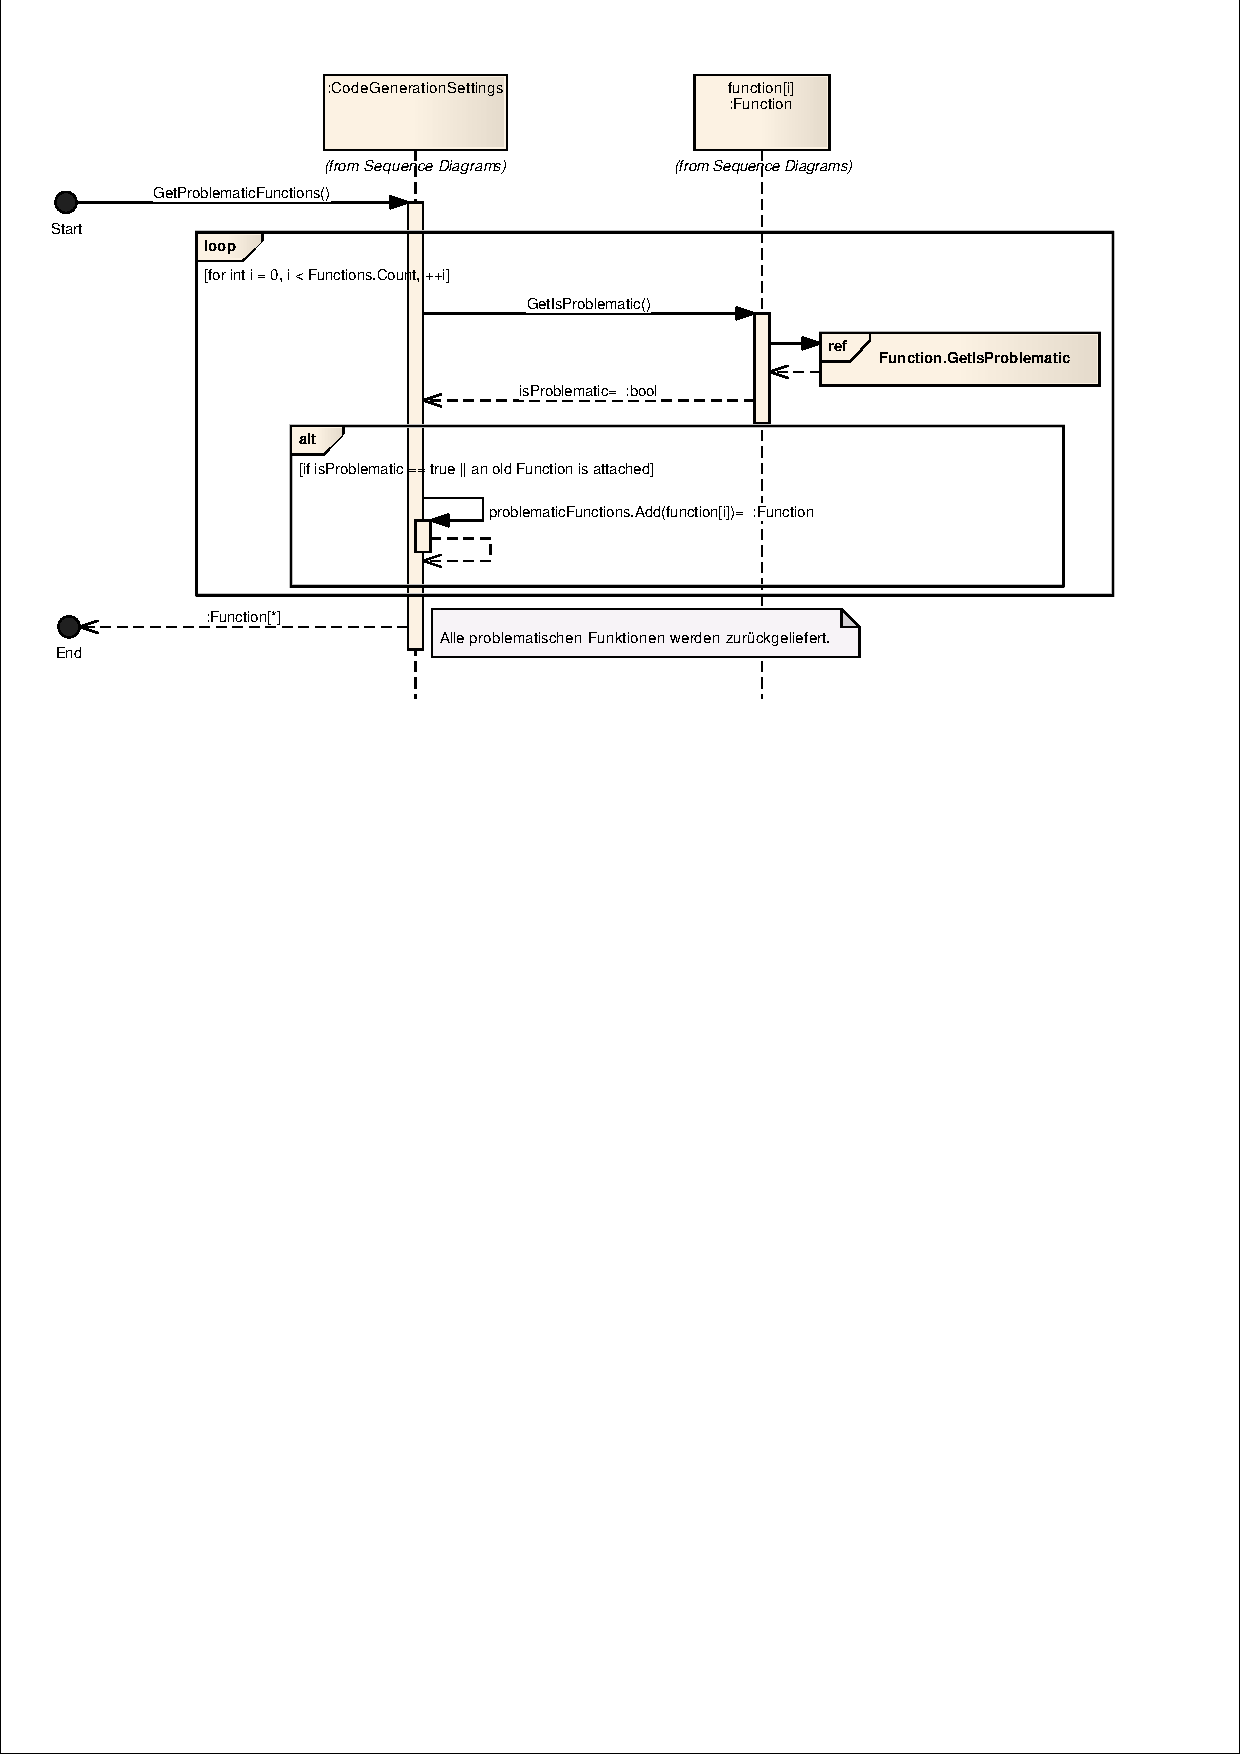
\includegraphics[trim = 1mm 180mm 1mm 1mm, clip, scale=0.7]{images/CodeGen_GetProblematicFunctions.pdf}
\caption{Sequenzdiagramm zum Auslesen aller problematischer Funktionen}\label{fig:cgGetPFunc}
\end{figure}

\begin{figure}[htp]
\centering
%trim=l b r t  	This option will crop the imported image by l from the left, b from the bottom, r from the right, and t  from the top. Where l, b, r and t are lengths. 
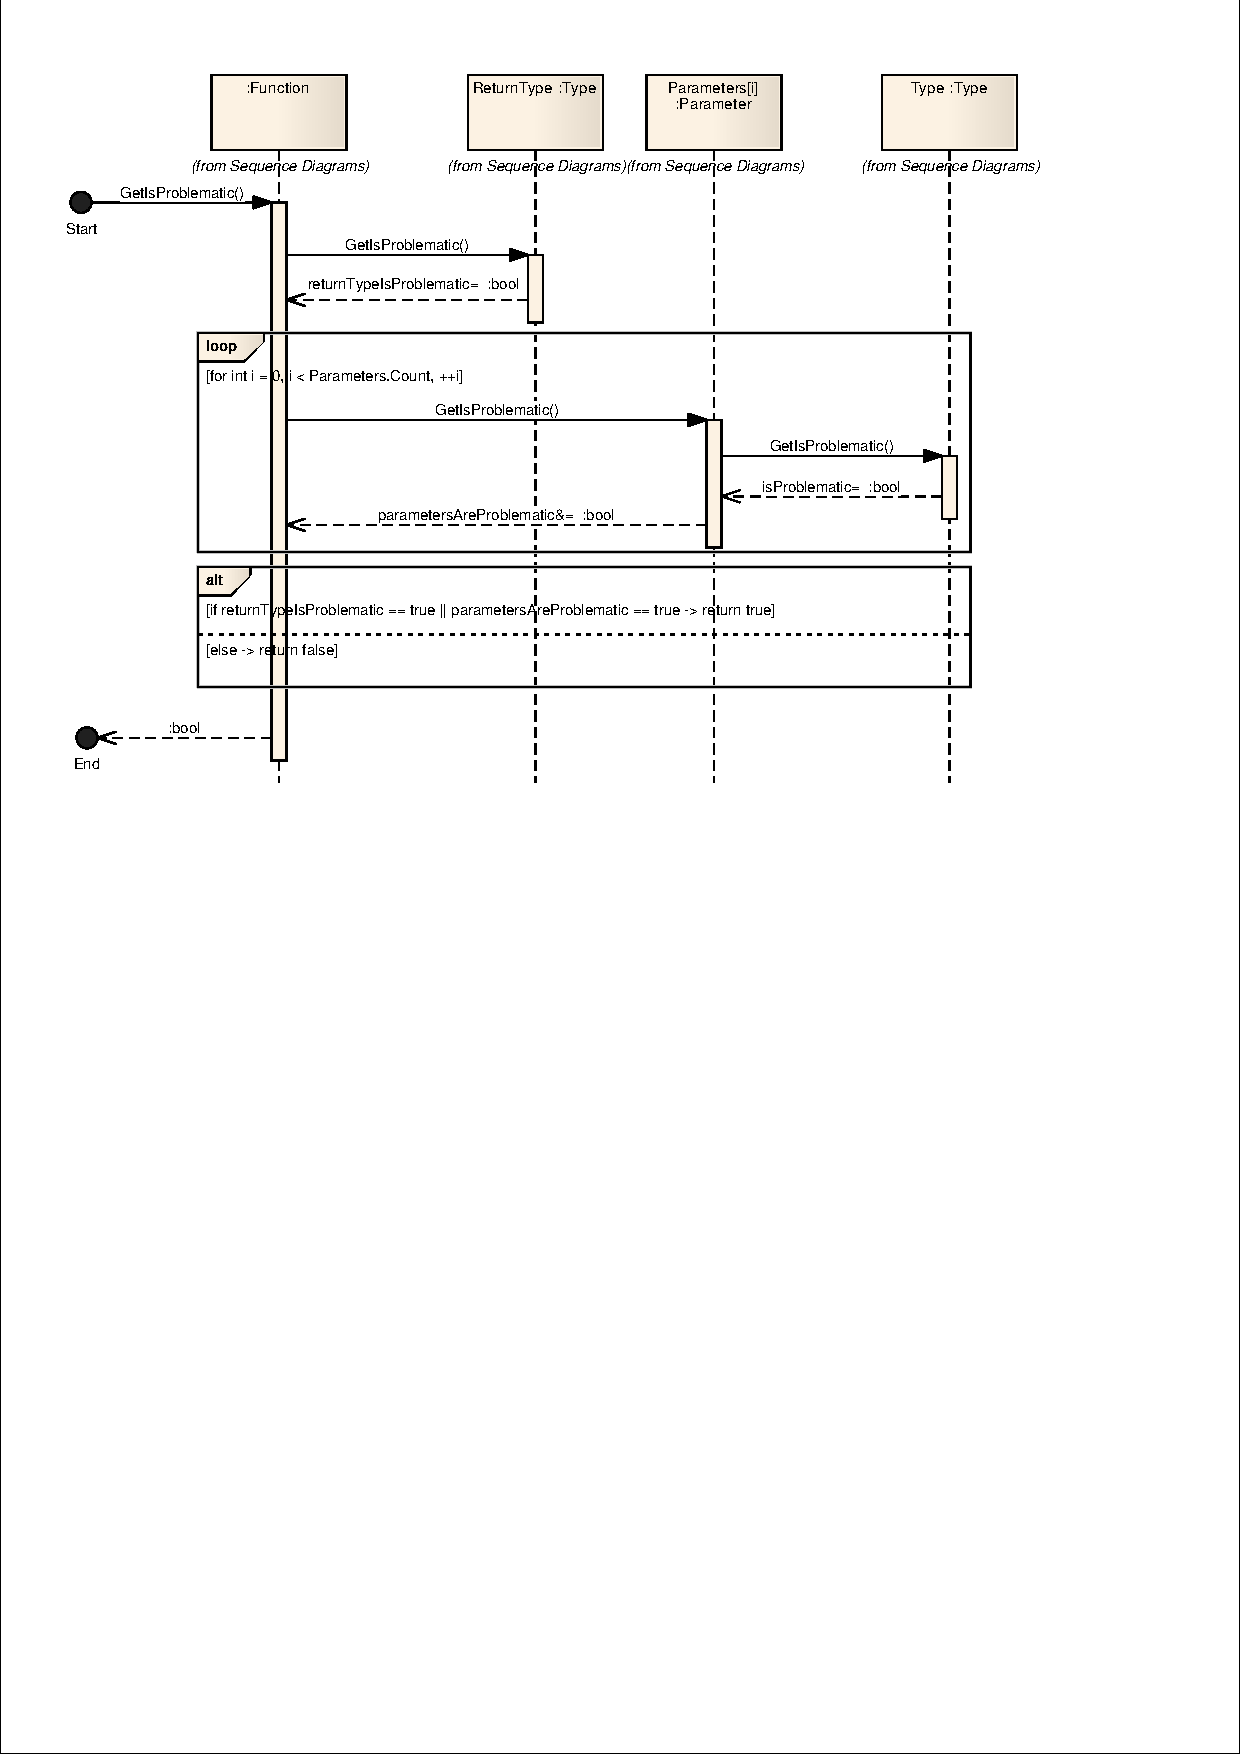
\includegraphics[trim = 1mm 165mm 20mm 1mm, clip, scale=0.7]{images/CodeGen_GetIsProblematic.pdf}
\caption{Sequenzdiagramm f�r das \emph{Property} \texttt{Function.IsProblematic}}\label{fig:cgIsProb}
\end{figure}

\begin{figure}[htp]
\centering
%trim=l b r t  	This option will crop the imported image by l from the left, b from the bottom, r from the right, and t  from the top. Where l, b, r and t are lengths. 
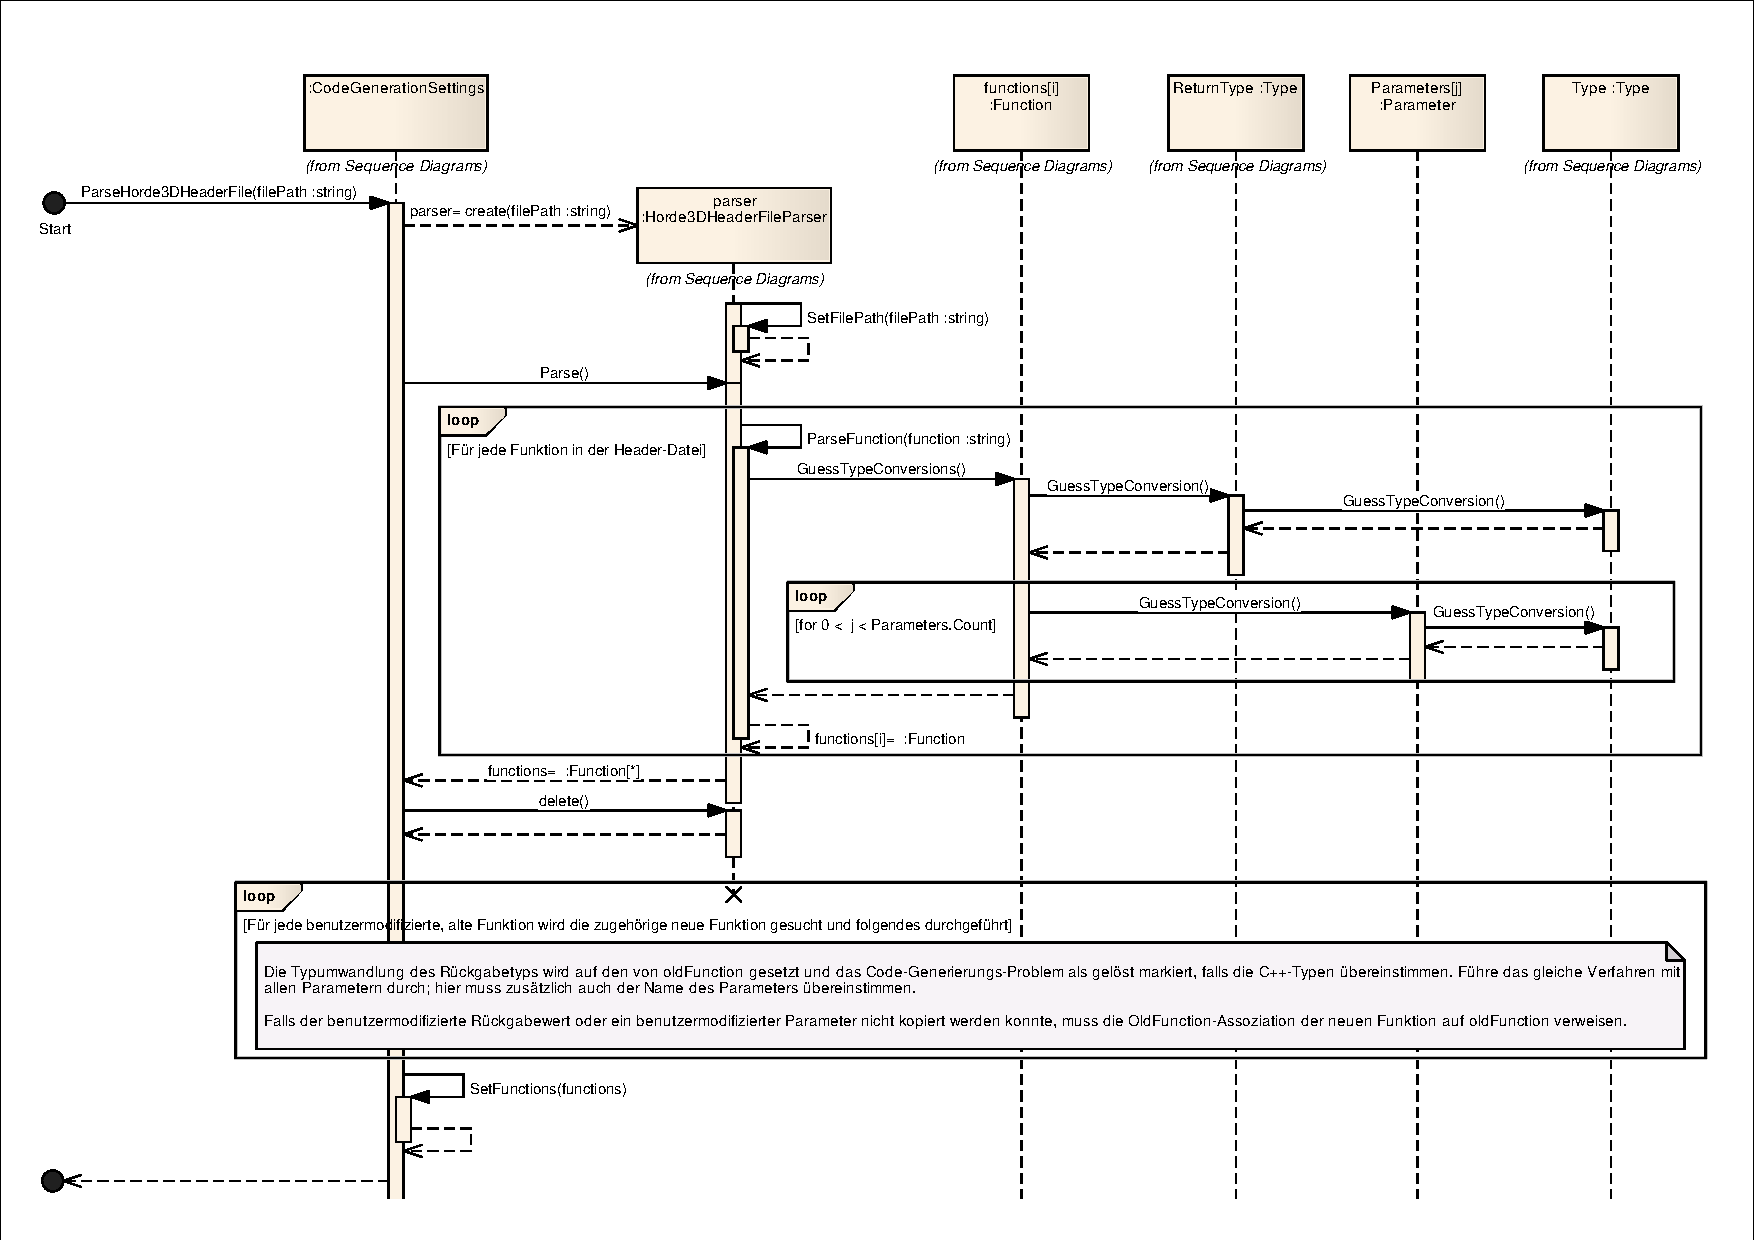
\includegraphics[trim = 1mm 1mm 1mm 1mm, clip, angle = 90, scale=0.7]{images/CodeGen_Parse.pdf}
\caption{Sequenzdiagramm f�r das Parsen der \emph{Header}-Datei}\label{fig:cgParse}
\end{figure}

